\documentclass[12pt,a4paper]{article}
\usepackage{preamble}

\hypersetup{pdftitle={Математическая физика — Практика}}

\begin{document}
% !TEX root = MathPhys.tex
\renewcommand{\notesuniversity}{Санкт-Петербургский государственный университет}
\renewcommand{\notesfaculty}{Факультет математики и механики}
\renewcommand{\notestitle}{Математическая физика}
\renewcommand{\notessubtitle}{Практика}
\renewcommand{\notesauthor}{}


\notesmaketitle


\tableofcontents

\newpage


% =====================================================================
\section{Практика 1}
\renewcommand{\notesheader}{Математическая физика \(\cdot\) Практика 1 \(\cdot\) 04.09}
% =====================================================================

\subsection{Пространство тест-функций \texorpdfstring{$\DD(\Omega)$}{D(Omega)}}

Пусть \(\Omega\) --- область. \(X\) --- пространство функций.
\(X' = X^*\) --- пространство линейных непрерывных функционалов
(по умолчанию со \(*\)-слабой топологией).

\[
\begin{array}{ccc}
X & & X' \\[4pt]
L_1(\Omega) & & L_\infty(\Omega) \\
\cup & & \cap \\
L_p(\Omega) & & L_{p'}(\Omega) \\
\cup & & \cap \\
C_0(\Omega) & & \mathcal{M}(\Omega) \\
\cup & & \cap \\
\dots & & \ldots
\end{array}
\]
где \(p' = \dfrac{p}{p-1}\), а \(\mathcal{M}(\Omega)\) --- пространство
конечных борелевских зарядов.

\remm{}{Чем беднее \(X\), тем богаче \(X'\).}

\exr{}{
Пусть \(X\), \(Y\) --- топологические векторные пространства,
\(X \hookrightarrow Y\), где \(\hookrightarrow\) такое, что
\(\exists A \colon X \to Y\), где \(A\) линейно, непрерывно и инъективно,
при этом \(X\) всюду плотно в \(Y. \) Тогда \(Y^* \hookrightarrow X^*\).
}

\dfn{Пространство тест-функций}{
\[
\DD(\Omega) \triangleq C_0^\infty(\Omega).
\]
}

\dfn{Понятие сходимости в $\DD(\Omega)$}{
\[
\phi_k \to \phi
\text{ в }\DD(\Omega)
\stackrel{\triangle}{\Longleftrightarrow}
\begin{cases}
1.\ \forall \alpha\ \ D^\alpha \phi_k \rightrightarrows D^\alpha \phi, \\[2pt]
2.\ \exists K\,\text{--- компакт} : \forall k \supp \phi_k \subset K \subset \Omega.
\end{cases}
\]
}

\remm{}{Пространство $\DD'(\Omega) = (\DD(\Omega))^*$ называется пространством обобщённых функций, его мы определим чуть позже.}

\exr{}{
Привести 2 топологических пространства с одинаковой сходимостью 
(Богачев В.\,И. ``Основы теории мер'', Том 2, стр.~70).
}

\exr{}{
Показать, что такая сходимость не может быть порождена метрикой.
}

\remm{}{
Схему вложений можно дополнить следующим образом:
\[
\begin{array}{ccc}
X & & X' \\[4pt]
L_1(\Omega) & & L_\infty(\Omega) \\
\cup & & \cap \\
L_p(\Omega) & & L_{p'}(\Omega) \\
\cup & & \cap \\
C_0(\Omega) & & \mathcal{M}(\Omega) \\
\cup & & \cap \\
C_0^\infty(\Omega) & & \DD'(\Omega)
\end{array}
\]
}


\stat{}{
\(C_0^\infty(\Omega)\) всюду плотно в \(L_p(\Omega)\) для всех \(p < \infty\).
}

\prf{
Пусть \(f \in L_p\), выберем компакт $K \subset \Omega$ так, чтобы $\|f - f\chi_K\|_p < \epsilon$.
Возьмем аппроксимативную единицу $\omega_n$ и построим функции $g_n \in C_0^{\infty}(\Omega)$:
\[
g_n = (f\cdot\chi_K) * \omega_n \xlongrightarrow{n} f\cdot\chi_K,
\]
\[
\|f - f\cdot\chi_K * \omega_n\|_{L_p}
\le
\|f - f\cdot\chi_K\|_{L_p}
+
\|f\cdot\chi_K - f\cdot\chi_K * \omega_n\|_{L_p}.
\]
}

\remm{}{В этой топологии (порожденной $L_p$-нормой) секвенциальная сходимость равносильна просто сходимости.}


% ---------------------------------------------------------------------
\subsection{Непрерывные операции в \texorpdfstring{\(\DD(\Omega)\)}{D(Omega)}}


\subsubsection{Умножение на \(C^\infty\)-функции}
Пусть у нас $
a \in C^\infty(\Omega), f \in \DD(\Omega),$ $$ A \colon \DD(\Omega) \to \DD(\Omega):\
f \mapsto a \cdot f
$$
оно линейно и непрерывно.

\remm{Напоминание}{
Линейный оператор $A: X \to Y$ непрерывен тогда и только тогда, когда он сохраняет сходимость в нуле:
$$
f_k \xrightarrow{X} 0 \implies A f_k \xrightarrow{Y} 0 \quad \text{при } k \to \infty
$$
Поэтому для доказательства непрерывности оператора в $\mathcal{D}(\Omega)$ мы обязаны проверить, что образ последовательности $A f_k$ удовлетворяет всем условиям сходимости целевого пространства.
}

\prf{
Пусть \(f_k \to 0\) в \(\DD(\Omega) \Rightarrow a f_k \to 0\) в \(\DD(\Omega)\). Проверим два условия сходимости для последовательности $a f_k$.
$$\supp(a f_k) \subset \supp f_k \subset K.$$ Здесь $K$ --- это тот самый единый компакт из определения сходимости $f_k \to 0$.

Распишем производную порядка \(\alpha\) от произведения: 
\[
D^{\alpha }(af_{k})= \text{лин. комбинация } \; D^{\beta }a\cdot D^{\alpha -\beta }f_{k},
\]
поскольку $D^{\beta }a$ непрерывны, на компакте $K$ они ограничены. 
А так как $f_k \xrightarrow{\mathcal{D}} 0$, 
то $D^{\alpha - \beta} f_k \rightrightarrows 0$ при $k \to \infty$. 

Следовательно, вся линейная комбинация равномерно стремится к нулю: $$D^\alpha(a f_k) \rightrightarrows 0.$$
}

\remm{}{
Формула Лейбница для мультииндексов: 
\[
D^{\alpha }(af_{k})=\sum _{\beta \le \alpha }\binom{\alpha}{\beta}D^{\beta }a\cdot D^{\alpha -\beta }f_{k},
\]
}

\dfn{}{
Функции \(\phi\) такие, что \(\phi \cdot X \subset X\), называют
мультиприлкаторами пространства \(X\).
}

\ex{Пространства и их мультипликаторы}{
\[
L_p(\Omega):\ L_\infty(\Omega)
\]
\[
C(\Omega):\ C(\Omega)
\]
\[
\DD(\Omega):\ C^\infty(\Omega)
\]
}

\subsubsection{Дифференцирование}
Оператор дифференцирования $D^\alpha$ является линейным и непрерывным в $\mathcal{D}(\Omega)$, поскольку функции пространства бесконечно гладкие, а взятие производных не расширяет их носители:
$$
D^\alpha : \mathcal{D}(\Omega) \to \mathcal{D}(\Omega) : f \mapsto D^\alpha f$$
\prf{
Пусть $f_k \xrightarrow{\mathcal{D}} 0$ при $k \to \infty$. Дифференцирование не расширяет носитель функции, поэтому $$\text{supp}(D^\alpha f_k) \subset \text{supp } f_k \subset K.$$ Все носители производных остаются в том же едином компакте $K \subset \Omega$.

Для любого мультииндекса $\beta$ рассмотрим производную порядка $\beta$ от нашей новой последовательности:
$$
D^\beta(D^\alpha f_k) = D^{\alpha + \beta} f_k.
$$
Поскольку последовательность $f_k$ сходилась к нулю в $\mathcal{D}(\Omega)$, её производные любого порядка равномерно стремились к нулю на $K$. Значит, и $D^{\alpha + \beta} f_k \rightrightarrows 0$ при $k \to \infty$.

Следовательно, $D^\alpha f_k \xrightarrow{\mathcal{D}} 0$, что и доказывает секвенциальную непрерывность оператора дифференцирования.
}

\subsubsection{Замена переменной}

Пусть \(\Omega_1, \Omega_2 \subset \mathbb{R}^n\) --- две области, и задан \(C^\infty\)-диффеоморфизм \(\Phi: \Omega_2 \to \Omega_1\) (якобиан которого, очевидно, нигде не обращается в нуль: \(\det |\Phi'| \neq 0\)).

\begin{center}
\begin{tikzpicture}[scale=1.05, baseline=(current bounding box.center)]
  \draw[black, thick] (0,0) ellipse (1.45cm and 0.9cm);
  \node at (0,0) {\(\Omega_2\)};
  \draw[-{Stealth}, black, thick] (1.85,0.12) -- (3.35,0.12);
  \node[above] at (2.6,0.12) {\(\Phi\)};
  \draw[black, thick] (5.2,0) ellipse (1.45cm and 0.9cm);
  \node at (5.2,0) {\(\Omega_1\)};
\end{tikzpicture}
\captionof{figure}{Диффеоморфизм \(\Phi\)}
\end{center}

Определим оператор замены переменной (композиции):
\[
A: \mathcal{D}(\Omega_1) \to \mathcal{D}(\Omega_2) : f \mapsto f \circ \Phi
\]

Данный оператор, очевидно, линеен. Докажем его секвенциальную непрерывность. 

Пусть \(f_k \xrightarrow{\mathcal{D}(\Omega_1)} 0\) при \(k \to \infty\). Покажем, что \(f_k \circ \Phi \xrightarrow{\mathcal{D}(\Omega_2)} 0\), проверив два условия сходимости:

По определению сходимости в \(\mathcal{D}(\Omega_1)\), существует единый компакт \(K \subset \Omega_1\), содержащий носители всех функций: \(\text{supp } f_k \subset K\). 
Поскольку отображение \(\Phi\) непрерывно, прообраз компакта \(K' \triangleq \Phi^{-1}(K)\) является компактом в области \(\Omega_2\). Тогда для носителей преобразованных функций выполняется включение:
\[
\text{supp}(f_k \circ \Phi) \subset \Phi^{-1}(\text{supp } f_k) \subset \Phi^{-1}(K) = K' \subset \Omega_2
\]
Таким образом, все носители функций \(f_k \circ \Phi\) зажаты внутри общего компакта \(K'\).

По правилу дифференцирования сложной функции, частная производная имеет вид:
\[
D_i(f_k \circ \Phi)(x) = \sum_{j=1}^n (D_j f_k)(\Phi(x)) \cdot \frac{\partial \Phi_j}{\partial x_i}(x)
\]
Поскольку \(\Phi \in C^\infty\), функции \(\frac{\partial \Phi_j}{\partial x_i}\) непрерывны и, следовательно, ограничены на компакте \(K'\). Так как \(f_k \xrightarrow{\mathcal{D}} 0\), их производные равномерно стремятся к нулю: \(D_j f_k \rightrightarrows 0\) на \(K\) при \(k \to \infty\). 
Из чего вытекает, что вся сумма равномерно сходится к нулю на \(K'\):
\[
D_i(f_k \circ \Phi) \rightrightarrows 0 \quad \text{при } k \to \infty
\]
Аналогично по индукции рассуждение верно для производных любого порядка \(\alpha\).

Следовательно, оператор замены переменной непрерывен из \(\mathcal{D}(\Omega_1)\) в \(\mathcal{D}(\Omega_2)\).




% ---------------------------------------------------------------------
\subsection{Пространство обобщённых функций \texorpdfstring{\(\DD'(\Omega)\)}{D'(Omega)}}

\dfn{Пространство обобщённых функций}{
    Пространством обобщённых функций \(\DD'(\Omega)\) называется пространство всех
    линейных непрерывных функционалов на \(\DD(\Omega)\):
    $$\DD'(\Omega) \triangleq (\DD(\Omega))^*.$$

    То есть элемент \(\widetilde{f} \in \DD'(\Omega)\) --- это линейный непрерывный функционал,
    который берет тест-функцию \(\phi \in \DD(\Omega)\) и сопоставляет ей число \(\widetilde{f}(\phi) \triangleq \langle \widetilde{f}, \phi \rangle\),
    при этом:
    \begin{enumerate}
        \item \(\langle \widetilde{f}, c_1 \phi_1 + c_2 \phi_2 \rangle = c_1 \langle \widetilde{f}, \phi_1 \rangle + c_2 \langle \widetilde{f}, \phi_2 \rangle\) (линейность),
        \item Если \(\phi_k \to \phi\) в \(\DD(\Omega)\), то \(\langle \widetilde{f}, \phi_k \rangle \to \langle \widetilde{f}, \phi \rangle\) (непрерывность).
    \end{enumerate}
}

\remm{Напоминание}{Алгебраический смысл: угловые скобки $\langle \widetilde{f}, \phi \rangle$ представляют собой каноническое билинейное спаривание между пространством тест-функций $\DD$ и сопряженным пространством линейных непрерывных функционалов $\DD'$.
}

Далее рассмотрим несколько примеров обобщённых функций.

\subsubsection{Регулярные функции \(L_1^{\loc}\)}

\dfn{Пространство локально интегрируемых функций}{
\[
L_1^{\loc}(\Omega)
\triangleq
\bigl\{
f\text{ измерима}:\
f \in L_1(K)\
\forall K \subset \Omega\text{ --- компакт}
\bigr\}.
\]
}

\stat{}{
    Если \(f \in L_1^{\text{loc}}(\Omega)\), то определяемый ею функционал 
    \[
    \langle \widetilde{f}, \phi \rangle \triangleq \int_{\Omega} f(x)\phi(x) \, dx
    \]
    является линейным непрерывным функционалом над \(\mathcal{D}(\Omega)\) (то есть \(\widetilde{f} \in \mathcal{D}'(\Omega)\)).
}

\prf{
Корректность определения: поскольку \(\phi \in \mathcal{D}(\Omega)\) финитна, её носитель \(\text{supp } \phi = K_0\) является компактом в \(\Omega\). Тогда интеграл берется по множеству конечной меры, где \(\phi\) ограничена, а \(f \in L_1(K_0)\). Следовательно, интеграл гарантированно сходится и принимает конечное числовое значение.

Линейность напрямую следует из линейных свойств интеграла Лебега:
\[
\langle \widetilde{f}, c_1\phi_1 + c_2\phi_2 \rangle = \int_{\Omega} f(c_1\phi_1 + c_2\phi_2) \, dx = c_1\langle \widetilde{f}, \phi_1 \rangle + c_2\langle \widetilde{f}, \phi_2 \rangle
\]

Непрерывность: пусть последовательность \(\phi_k \xrightarrow{\mathcal{D}} 0\) при \(k \to \infty\). По определению сходимости в \(\mathcal{D}(\Omega)\), существует единый общий компакт \(K \subset \Omega\), такой что \(\text{supp } \phi_k \subset K\) для всех \(k\), а сами функции равномерно стремятся к нулю: \(\max_{\Omega} |\phi_k| \to 0\).

Оценим модуль функционала:
\[
|\widetilde{f}(\phi_k)| = \left| \int_{K} f(x)\phi_k(x) \, dx \right| \le \int_{K} |f(x)| \cdot |\phi_k(x)| \, dx \le \max_{\Omega} |\phi_k| \int_{K} |f(x)| \, dx
\]
Поскольку \(f \in L_1^{\text{loc}}(\Omega)\), интеграл \(\int_{K} |f(x)| \, dx\) ограничен. Так как \(\max_{\Omega} |\phi_k| \to 0\), правая часть неравенства стремится к нулю при \(k \to \infty\). Непрерывность доказана.
}

\lem{}{
Если \(f \in L_1^{\loc}(\Omega)\) и
\(\int_{\Omega} f\cdot\phi = 0\) для всех
\(\phi \in \DD(\Omega)\), то \(f = 0 \text{ п.в.}\) на \(\Omega\).
}

\remm{}{
Это гарантирует инъективность отображения $L_1^{\loc}(\Omega) \to \DD'(\Omega) : f \mapsto \widetilde{f}$.
Если регулярный функционал тождественно равен нулю в пространстве обобщенных функций $\mathcal{D}'(\Omega)$, то порождающая его функция также обязана быть нулевой:
\[
\widetilde{f} = 0 \text{ в } \mathcal{D}'(\Omega) \implies \int_{\Omega} f(x)\phi(x) \, dx = 0 \quad \forall \phi \in \mathcal{D}(\Omega) \implies f(x) = 0 \text{ п.в.}
\]
Значит, разные регулярные функции порождают разные обобщенные функции, что позволяет нам зафиксировать корректное каноническое вложение пространств:
\[
L_1^{\loc}(\Omega) \hookrightarrow \mathcal{D}'(\Omega), \quad \langle \widetilde{f}, \phi \rangle \triangleq \int_{\Omega} f(x)\phi(x) \, dx.
\]
}

\remm{}{
Далее буду отождествлять регулярные функции с порождаемыми ими обобщёнными функциями, то есть писать \(f \in L_1^{\loc}(\Omega) \subset \mathcal{D}'(\Omega)\) и опускать тильду над \(f\).
}

\subsubsection{Заряды \texorpdfstring{\(\mathcal{M}_{\loc}(\Omega)\)}{M loc(Omega)}}

По аналогии с локально интегрируемыми функциями, в пространство обобщенных функций можно вложить пространство локально конечных регулярных борелевских зарядов.

\remm{Напоминание}{Если область \(\Omega \subset \mathbb{R}^n\), то любой конечный борелевский заряд автоматически обладает свойством регулярности.
}

\dfn{Пространство локально конечных зарядов}{
\[
\mathcal{M}_{\loc}(\Omega) \triangleq \{ \mu \text{ --- борелевский заряд} : |\mu|(K) < \infty \; \forall K \subset \Omega \text{ --- компакт} \}
\]
}

Каждому заряду \(\mu \in \mathcal{M}_{\loc}(\Omega)\) сопоставляется линейный непрерывный функционал \(\mu \in \mathcal{D}'(\Omega)\), действующий по правилу:
\[
\langle \mu, \phi \rangle \triangleq \int_{\Omega} \phi(x) \, d\mu(x) \quad \forall \phi \in \mathcal{D}(\Omega)
\]

\exr{}{Докажите, что данный функционал действительно непрерывен (\(\mu \in \mathcal{D}'(\Omega)\)), а отображение \(\mathcal{M}_{\loc}(\Omega) \to \mathcal{D}'(\Omega) : \mu \mapsto \mu\) является инъективным.
}

\ex{Функция Дирака}{
Она задается с помощью сосредоточенной в нуле вероятностной меры Дирака (дельта-меры):
\[
\delta(S) = \begin{cases} 1, & 0 \in S, \\ 0, & 0 \notin S. \end{cases}
\]
где \(S\) --- произвольное борелевское подмножество из \(\Omega\). 

Действие дельта-функционала на тест-функции \(\phi \in \mathcal{D}(\Omega)\) вычисляется через интеграл Лебега по этой мере и сводится к вычислению значения функции в нуле:
\[
\langle \delta, \phi \rangle = \int_{\Omega} \phi(x) \, d\delta(x) = \phi(0).
\]
}

\ex{Простой слой}{
\(\Sigma\) --- поверхность в \(\Omega\),
\(\mu\) --- мера на \(\Sigma\), индуцированная лебеговой мерой. 
\begin{center}
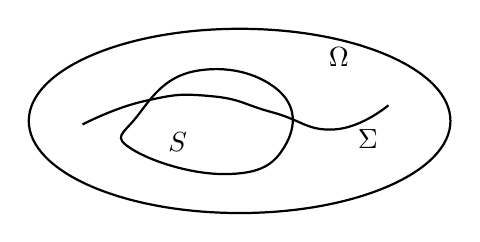
\begin{tikzpicture}[x=1.05cm, y=0.9cm, baseline=(current bounding box.center)]
  \draw[black, thick] (0,0) ellipse (2.55 and 1.3);
  \node[black] at (1.2,0.9) {\(\Omega\)};
  \draw[black, thick]
    plot[smooth cycle, tension=0.8]
    coordinates {
      (-1.25,0.05) (-0.55,0.7) (0.45,0.45)
      (0.55,-0.35) (-0.15,-0.75) (-1.3,-0.4)
    };
  \node[black] at (-0.75,-0.3) {\(S\)};
  \draw[black, thick]
    plot[smooth, tension=0.85]
    coordinates {
      (-1.9,-0.05) (-1.15,0.28) (-0.35,0.35)
      (0.4,0.12) (1.15,-0.12) (1.8,0.22)
    };
  \node[black, below] at (1.55,0.01) {\(\Sigma\)};
\end{tikzpicture}
\captionof{figure}{Схема области $\Omega$, подобласти $S$ и поверхности $\Sigma$}
\end{center}
Обобщенная функция простого слоя $\delta_{\Sigma} \in \mathcal{D}'(\Omega)$ определяется как мера
\[
\delta(S) = \mu(S \cap \Sigma)
\]
а её действие на функцию $\phi \in \mathcal{D}(\Omega)$ задается правилом:
\[
\langle \delta_\Sigma,\, \phi \rangle
=
\int_\Sigma \phi\,d\Sigma.
\]
}

\exr{}{Доказать, что дельта-функция Дирака \(\delta\) --- не является регулярной.}

% ---------------------------------------------------------------------
\subsection{Носитель обобщённой функции}

Пусть \(f \in \DD'(\Omega)\).

\dfn{}{
\(\supp f\) --- наименьшее замкнутое множество, вне которого \(f = 0\).
}

Далее определим, что же значит, что \(f = 0\) на множестве:
\dfn{}{
\(f = 0\) на \(\Omega' \text{-- откр.}\) \(\subset \Omega\)
\(\Leftrightarrow\)
\(\langle f,\, \phi \rangle = 0\)
для всех \(\phi \in \DD(\Omega)\) с \(\supp\phi \subset \Omega'\).
}

\rem{}{
$
f = 0\text{ на }\Omega
\iff
f = 0\text{ в }\DD'(\Omega)
\iff
\langle f,\, \phi \rangle = 0
\quad \forall \phi \in \DD(\Omega).
$
}

\lem{}{
Если \(f = 0\) на \(\Omega_\alpha\), то \(f = 0\) на
\(\bigcup_\alpha \Omega_\alpha\).
}

\prf{
\(\phi \in \DD\bigl(\bigcup_\alpha \Omega_\alpha\bigr)\),
\(\langle f,\, \phi \rangle = 0\)?
\[
K = \supp\phi,
\qquad
K \subset \bigcup_\alpha \Omega_\alpha
\]
\[
K \subset \bigcup_{i=1}^N \Omega_{\alpha_i}.
\]
\(\exists \{\eta_i\}_{i=1}^N\) --- разбиение единицы, т.е.
\[
\sum_{i=1}^N \eta_i = 1
\quad\text{на }K
\]
\[
\supp\eta_i \subset \Omega_{\alpha_i}.
\]
\begin{align*}
\langle f,\, \phi \rangle
&=
\Bigl\langle f,\, \Bigl(\sum_{i=1}^N \eta_i\Bigr)\phi \Bigr\rangle
=
\sum_{i=1}^N
\overbrace{
  \bigl\langle
    f,\,
    \underbrace{\eta_i\phi}_{\supp\subset\Omega_{\alpha_i}}
  \bigr\rangle
}^{=0}
= 0.
\end{align*}
}

\dfn{}{
\(f = g\) на \(\Omega_1\), если \(f - g = 0\) на \(\Omega_1\).
}

\dfn{}{
\(\operatorname{sing\,supp} f\) --- наименьшее замкнутое множество,
вне которого \(f\) совпадает с какой-то \(C^\infty\)-функцией.
}

\ex{}{
\[
\supp\delta = \{0\},
\qquad
\operatorname{sing\,supp}\delta = \{0\}.
\]
\[
\supp\delta_\Sigma
=
\operatorname{sing\,supp}\delta_\Sigma
=
\Sigma.
\]
}

\exr{}{
Если \(f\) --- заряд или регулярная функция, то \(\supp f\) в этом смысле
совпадает с \(\supp f\) в стандартном смысле.
}

% ---------------------------------------------------------------------
\subsection{Операции над обобщёнными функциями}

\subsubsection{Умножение на \(C^\infty(\Omega)\)-функции}
\(a \in C^\infty(\Omega)\), \(f \in \DD'(\Omega)\), хотим определить
\(a \cdot f\).
Рассмотрим \(f \in L_1^{\loc}(\Omega)\):
\[
\langle af,\, \phi \rangle
=
\int_\Omega af\,\phi
=
\int_\Omega f(a\phi)
=
\langle f,\, a\phi \rangle.
\]

\dfn{}{
\(f \in \DD'(\Omega)\), \(a \in C^\infty(\Omega)\)
\[
\langle af,\, \phi \rangle
:=
\langle f,\, a\phi \rangle,
\qquad
a\phi \in C_0^\infty(\Omega).
\]
}
Это корректно, линейно и непрерывно. \(f(\phi)\), \(\phi \mapsto a\phi\).

\ex{}{
\(a \in C^\infty\)
\[
\langle a\delta,\, \phi \rangle
=
\langle \delta,\, a\phi \rangle
=
a(0)\,\phi(0)
=
a(0)\,\langle \delta,\, \phi \rangle
\]
\[
a(x)\,\delta(x) = a(0)\,\delta(x)
\]
\[
f \xrightarrow{A} a \cdot f
\]
\(\delta\) --- это обобщённая функция, собственная функция \(A\).
}

\exr{}{
\(\eta \in C^\infty(\Omega)\) и \(\eta \equiv 1\) на \(\supp f\),
\(f \in \DD(\Omega)\). Тогда \(\eta f = f\).
}

\subsubsection{Замена координат}
\(\Phi\) --- диффеоморфизм \(\Phi \colon \Omega \to \Omega_1\).
Хотим определить \(f \circ \Phi\) для \(f \in \DD'(\Omega_1)\).
Рассмотрим \(f \in L_1^{\loc}(\Omega)\):
\begin{align*}
\langle f \circ \Phi,\, \phi \rangle
&=
\int f\bigl(\Phi(x)\bigr)\,\phi(x)\,dx \\
&\stackrel{y=\Phi(x)}{=}
\int_\Omega f(y)\,
\frac{\phi(\Phi^{-1}(y))}{|\det\Phi'(y)|}\,dy \\
&=
\biggl\langle
    f,\,
    \frac{\phi \circ \Phi^{-1}}{|\det\Phi|}
\biggr\rangle
\in \DD'(\Omega_1).
\end{align*}

\dfn{}{
\[
\langle f \circ \Phi,\, \phi \rangle
:=
\biggl\langle
    f,\,
    \frac{\phi \circ \Phi^{-1}}{|\det\Phi|}
\biggr\rangle
\]
\[
\phi \circ \Phi^{-1} \in C_0^\infty(\Omega_1),
\qquad
\frac{1}{|\det\Phi|}.
\]
}
Это определение корректно, линейно и непрерывно
(композиция непрерывных отображений).

\ex{}{
\[
\langle \delta(x-x^0),\, \phi \rangle
=
\biggl\langle
    \delta(x),\,
    \frac{\phi(x+x^0)}{1}
\biggr\rangle
=
\phi(x^0)
\]
\[
a(x) \cdot \delta(x-x^0)
=
a(x^0) \cdot \delta(x-x^0).
\]
\(\delta(x-x^0)\) --- собственная функция для \(A \colon f \mapsto af\).
}

\ex{}{
\(\lambda \neq 0\)
\[
\langle \delta(\lambda x),\, \phi(x) \rangle
=
\biggl\langle
    \delta(x),\,
    \frac{\phi\bigl(\tfrac{x}{\lambda}\bigr)}{|\lambda|^n}
\biggr\rangle
=
\frac{\phi(0)}{|\lambda|^n}.
\]
\[
\Phi(x) = \lambda x
\]
\[
\Phi'(x)
=
\begin{pmatrix}
\lambda & & \\
& \ddots & \\
& & \lambda
\end{pmatrix}
\]
Таким образом
\[
\delta(\lambda x)
=
\frac{1}{|\lambda|^n}\,\delta(x),
\]
то есть \(\delta\) --- положительная однородная функция порядка \(n\).
}

\ex{}{
\(U\) --- ортогональная матрица, \(\delta\)-функция инвариантна
относительно поворотов.
\[
\delta(Ux) = \delta(x)
\]
\[
\delta(x)
=
\begin{cases}
\infty, & x = 0, \\
0, & x \neq 0.
\end{cases}
\]
}

\exr{}{
\(a \in C^\infty(\Omega)\), \(f \in \DD'(\Omega)\),
\(\Phi\) --- диффеоморфизм \(\Omega \to \Omega_1\). Тогда
\[
(af)\bigl(\phi(x)\bigr)
=
a\bigl(\phi(x)\bigr)\,f\bigl(\phi(x)\bigr).
\]
}

\subsubsection{Дифференцирование}
\(D^\alpha f\) ---?
Рассмотрим \(f \in C^1(\Omega)\):
\[
\langle D_i f,\, \phi \rangle
=
\int_\Omega D_i f\,\phi
=
-\int_\Omega f\, D_i\phi
=
-\langle f,\, D_i\phi \rangle.
\]

\dfn{}{
\(f \in \DD'(\Omega)\)
\[
\langle D_i f,\, \phi \rangle
=
-\langle f,\, D_i\phi \rangle
\]
\[
\langle D^\alpha f,\, \phi \rangle
=
(-1)^{|\alpha|}\,
\langle f,\, D^\alpha\phi \rangle.
\]
}

Определение корректно.

\remm{}{Где все функции дифференцируемые!!!}


\exr{}{
\(D^\alpha D^\beta f = D^\beta D^\alpha f = D^{\alpha+\beta} f\).
}

\exr{}{
Правило Лейбница
\(D_i(a \cdot f) = D_i a \cdot f + a D_i f\).
}

\exr{}{
\(\supp D^\alpha f \subset \supp f\) и привести пример, когда нет равенства.
}

\exr{}{
\(\operatorname{sing\,supp} D^\alpha f \subset \operatorname{sing\,supp} f\)
и привести пример, когда нет равенства.
}

\pagebreak
% =====================================================================
\section{Практика 2}
\renewcommand{\notesheader}{Математическая физика \(\cdot\) Практика 2 \(\cdot\) 11.09}
% =====================================================================

\remm{Напоминание}{
На прошлой паре мы уже ввели:
\[
C^\infty(\Omega) = \DD(\Omega),
\qquad
\text{\(\Omega\) --- область в \(\R^n\).}
\]
Сходимость в \(\DD(\Omega)\):
\[
u_k \to u
\quad\iff\quad
\begin{cases}
D^\alpha u_k \rightrightarrows D^\alpha u, \\[2pt]
\supp u_k \subset K\text{ --- компакт}.
\end{cases}
\]
Обобщённая производная:
\[
\langle D^\alpha u,\, \phi \rangle
= (-1)^{|\alpha|}\,
\langle u,\, D^\alpha \phi \rangle.
\]
}

\remm{}{В такой топологии непрерывность равносильна секвенциальной непрерывности.}

% ---------------------------------------------------------------------
\subsection{Примеры}

\ex{Дифференциальный оператор}{
Пусть \(P\) --- многочлен от \(n\) переменных,
\[
Lu = P(D)u
= \sum_{|\alpha| \le m} a_\alpha(x)\, D^\alpha u,
\qquad
a_\alpha \in C^\infty(\Omega).
\]
Тогда
\begin{align*}
\langle P(D)u,\, \phi \rangle
&= \Bigl\langle
    \sum_{|\alpha| \le m} a_\alpha(x)\, D^\alpha u(x),\,
    \phi(x)
\Bigr\rangle \\
&= \sum_{k \le m}
    \Bigl\langle
        \sum_{|\alpha|=k} a_\alpha(x)\, D^\alpha u,\,
        \phi
    \Bigr\rangle
= \bigl\langle u,\, L^*\phi \bigr\rangle,
\end{align*}
где формально сопряжённый оператор
\[
L^*\phi
= \sum_{k \le m} (-1)^k
    \sum_{|\alpha|=k}
        D^\alpha\bigl(a_\alpha \phi\bigr).
\]
В слабой форме, если \(Lu = f\),
\[
\int_\Omega Lu \cdot \phi
= \int_\Omega f\,\phi,
\qquad
\int_\Omega u\, L^*\phi
= \int_\Omega f\,\phi.
\]
}

\ex{Функция Хевисайда}{
Пусть \(n=1\) и
\(\Theta(x) = \chi_{[0,+\infty)}(x)\).
Найдём обобщённую производную \(\Theta'(x)\).
\begin{align*}
\langle \Theta',\, \phi \rangle
&= -\langle \Theta,\, \phi' \rangle
= -\int_0^\infty \phi'(x)\,dx.
\end{align*}
Так как \(\phi\) финитна, на \(+\infty\) она равна нулю, поэтому
\[
\langle \Theta',\, \phi \rangle
= \phi(0)
= \langle \delta,\, \phi \rangle.
\]
Итог:
\[
\Theta' = \delta.
\]
}

\ex{Производные дельта-функции}{
\[
\langle D^\alpha \delta,\, \phi \rangle
= (-1)^{|\alpha|}\, D^\alpha \phi(0).
\]
}

\exr{}{
Пусть \(f\) --- кусочно-гладкая функция на \(\R\).
Найти \(f' \in \DD'(\R)\).
\par\smallskip
\noindent\textit{Подсказка:} понадобится функция Хевисайда.
}

% =====================================================================
\subsection{Сингулярное ядро}

\lem{Локальная интегрируемость}{
\(\displaystyle \frac{1}{|x|^\alpha} \in L_1^{\loc}(\R^n)\),
если \(\alpha < n\).
}

\prf{
Нужно показать, что на любом компакте эта функция интегрируема:
\begin{align*}
\int_{B_R(0)} \frac{1}{|x|^\alpha}\,dx
&= \int_{S_1} \int_0^R \frac{r^{n-1}}{r^\alpha}\,dr
= |S_1|\, \frac{R^{n-\alpha}}{n-\alpha}
< \infty.
\end{align*}
}

\dfn{Сингулярное ядро}{
Пусть \(A \in C(S_1)\) и \(\displaystyle \int_{S_1} A = 0\).
Тогда
\[
\frac{A\bigl(\tfrac{x}{|x|}\bigr)}{|x|^n}
\]
называется \textit{сингулярным ядром}.
}

\remm{}{В общем случае такое ядро \(\notin L_1^{\loc}(\R^n)\).}

\stat{Главное значение}{
\[
\Bigl\langle
    \Pvf \frac{A\bigl(\tfrac{x}{|x|}\bigr)}{|x|^n},\,
    \phi
\Bigr\rangle
=
\vp \int_{\R^n}
    \frac{A\bigl(\tfrac{x}{|x|}\bigr)}{|x|^n}\,
    \phi(x)\,dx.
\]
}

\remm{}{Эта конструкция задаёт обобщённую функцию (оператор) из \(\DD'(\R^n)\).}

\remm{Напоминание}{По определению
\[
\vp \int_{\R^n}
    \frac{A\bigl(\tfrac{x}{|x|}\bigr)}{|x|^n}\,
    \phi(x)\,dx
=
\lim_{\epsilon \to 0}
\int_{\R^n \setminus B_\epsilon}
    \frac{A\bigl(\tfrac{x}{|x|}\bigr)}{|x|^n}\,
    \phi(x)\,dx.
\]
}

\remm{}{\(\Pvf\) (\textit{principal}) --- это то же самое, что \(\vp\) или \(\pv\).}

\prf{
Пусть \(\supp \phi \subset B_R\). Тогда
\begin{align*}
\Bigl\langle
    \frac{A\bigl(\tfrac{x}{|x|}\bigr)}{|x|^n},\,
    \phi
\Bigr\rangle
&=
\lim_{\epsilon \to 0}
\int_{B_R \setminus B_\epsilon}
    \frac{A\bigl(\tfrac{x}{|x|}\bigr)}{|x|^n}\,
    \phi(x)\,dx \\[4pt]
&=
\lim_{\epsilon \to 0}
\Biggl[
    \underbrace{
        \phi(0)
        \int_{B_R \setminus B_\epsilon}
            \frac{A\bigl(\tfrac{x}{|x|}\bigr)}{|x|^n}\,dx
    }_{
        =\;
        \displaystyle
        \Bigl(\int_{S_1} A\,dS\Bigr)
        \int_\epsilon^R r^{-1}\,dr
        = 0
    }
    +
    \int_{B_R \setminus B_\epsilon}
        \frac{\phi(x)-\phi(0)}{|x|^n}
        A\Bigl(\tfrac{x}{|x|}\Bigr)\,dx
\Biggr].
\end{align*}
Правое слагаемое оценивается так:
\[
\Biggl|
\int_{B_R}
    \frac{\phi(x)-\phi(0)}{|x|^n}
    A\Bigl(\tfrac{x}{|x|}\Bigr)\,dx
\Biggr|
\le
C \int_{B_R} \frac{\max|D\phi|\,|x|}{|x|^n}\,dx
\le
C \cdot \max|D\phi| \cdot R.
\]
По сути мы доказали, что
\[
\Bigl\langle
    \frac{A\bigl(\tfrac{x}{|x|}\bigr)}{|x|^n},\,
    \phi
\Bigr\rangle
=
\int_{B_R}
    \frac{\phi(x)-\phi(0)}{|x|^n}
    A\Bigl(\tfrac{x}{|x|}\Bigr)\,dx,
\]
где \(R\) таково, что \(\supp \phi \subset B_R\).

\remm{}{\(\vp \int f(x)\,dx = \int f(x)\,dx\), если \(f \in L_1\).}

Мы доказали, что функционал определён и линеен (линейность очевидна).
Осталось показать непрерывность.

Пусть \(\varphi_k \to 0\) в \(\DD(\R^n)\). Тогда
\[
\Biggl|
\Bigl\langle
    \frac{A\bigl(\tfrac{x}{|x|}\bigr)}{|x|^n},\,
    \varphi_k
\Bigr\rangle
\Biggr|
\le
C \cdot \max|D\varphi_k| \cdot R.
\]
Из \(\varphi_k \to 0\) следует \(D\varphi_k \to 0\), значит
\(\max|D\varphi_k| \to 0\), и поэтому
\[
\Biggl|
\Bigl\langle
    \frac{A\bigl(\tfrac{x}{|x|}\bigr)}{|x|^n},\,
    \varphi_k
\Bigr\rangle
\Biggr|
\xrightarrow{k\to\infty} 0.
\]
}

\remm{}{По сути мы определили \(\frac{1}{|x|^n}\) на всём \(\R^n\):
\[
\Pvf \frac{A\bigl(\tfrac{x}{|x|}\bigr)}{|x|^n}
=
\frac{A\bigl(\tfrac{x}{|x|}\bigr)}{|x|^n}
\quad\text{в }\R^n \setminus \{0\},
\]
то есть нашли продолжение ядра на всё \(\R^n\).}

% ---------------------------------------------------------------------
\ex{Производная радиального потенциала}{
Классически, вне нуля,
\[
D_i \Bigl(\frac{1}{|x|^\alpha}\Bigr)
= -\alpha\, \frac{x_i}{|x|^{\alpha+2}}.
\]
В смысле обобщённых функций разберём два случая.

\medskip
\noindent\textbf{1)}\ \(\alpha < n-1\).
\begin{align*}
\Bigl\langle D_i \frac{1}{|x|^\alpha},\, \phi \Bigr\rangle
&=
-\Bigl\langle \frac{1}{|x|^\alpha},\, D_i\phi \Bigr\rangle
=
-\int_{\R^n} \frac{D_i\phi}{|x|^\alpha}\,dx,
\end{align*}
поскольку \(\frac{1}{|x|^\alpha} \in L_1^{\loc}\) и задаёт регулярную
обобщённую функцию. Далее
\begin{align*}
&=
-\vp \int_{\R^n} \frac{D_i\phi}{|x|^\alpha}\,dx
=
\lim_{\epsilon\to 0}
\int_{\R^n \setminus B_\epsilon}
    \frac{D_i\phi}{|x|^\alpha}\,dx \\[3pt]
&=
\lim_{\epsilon\to 0}
\Biggl[
    \int_{\R^n \setminus B_\epsilon}
        \frac{-\alpha x_i}{|x|^{\alpha+2}}\,
        \phi(x)\,dx
    -
    \int_{S_\epsilon}
        \frac{\phi(x)}{|x|^\alpha}\,
        n_i\,dS
\Biggr].
\end{align*}
Поверхностный член исчезает:
\[
\Biggl|
\int_{S_\epsilon}
    \frac{\phi(x)}{|x|^\alpha}\, n_i\,dS
\Biggr|
\le
\frac{C\cdot \max|\phi|}{\epsilon^\alpha}\, |S_\epsilon|
=
C\cdot \max|\phi| \cdot \epsilon^{n-1-\alpha}
\xrightarrow{\epsilon\to 0} 0,
\]
так как \(\alpha < n-1\). Следовательно,
\[
\Bigl\langle D_i \frac{1}{|x|^\alpha},\, \phi \Bigr\rangle
=
\Bigl\langle
    -\frac{\alpha x_i}{|x|^{\alpha+2}},\,
    \phi
\Bigr\rangle.
\]

\medskip
\noindent\textbf{2)}\ \(\alpha = n-1\).
\begin{align*}
\Bigl\langle
    D_i\Bigl(\frac{1}{|x|^{n-1}}\Bigr),\,
    \phi
\Bigr\rangle
&=
\lim_{\epsilon\to 0}
\Biggl[
    \int_{\R^n \setminus B_\epsilon}
        \frac{-(n-1)x_i}{|x|^{n+1}}\,
        \phi(x)\,dx
    -
    \int_{S_\epsilon}
        \frac{\phi(x)}{|x|^{n-1}}\,
        n_i\,dS_\epsilon
\Biggr].
\end{align*}
Здесь
\(\frac{x_i}{|x|} = A\bigl(\tfrac{x}{|x|}\bigr)\)
и
\(\displaystyle \int_{S_1} A\bigl(\tfrac{x}{|x|}\bigr) = 0\),
поэтому объёмный член даёт
\[
\Bigl\langle
    \frac{-(n-1)\, A\bigl(\tfrac{x}{|x|}\bigr)}{|x|^n},\,
    \phi
\Bigr\rangle.
\]
Осталось показать, что поверхностный интеграл стремится к нулю.
Пусть \(n = \frac{x}{|x|}\), \(n_i = \frac{x_i}{|x|}\). Тогда
\begin{align*}
\Biggl|
\int_{S_\epsilon}
    \frac{\phi(x)}{\epsilon^{n-1}}\, n_i\,dS
\Biggr|
&=
\Biggl|
\frac{1}{\epsilon^{n-1}}
\Biggl(
    \int_{S_\epsilon} \phi(0)\, n_i\,dS
    +
    \int_{S_\epsilon} \bigl(\phi(x)-\phi(0)\bigr)\, n_i\,dS
\Biggr)
\Biggr| \\[3pt]
&\le
\frac{1}{\epsilon^{n-1}}
\int_{S_\epsilon} \max|D\phi|\, |x|\,dS
\le
C \cdot \max|D\phi| \cdot \epsilon
\xrightarrow{\epsilon\to 0} 0.
\end{align*}
(Первое слагаемое с \(\phi(0)\) обнуляется за счёт
\(\int_{S_\epsilon} n_i\,dS = 0\).)

Итог:
\[
D_i\Bigl(\frac{1}{|x|^{n-1}}\Bigr)
=
-(n-1)\,
\Pvf \frac{x_i}{|x|^{n+1}}.
\]
}

% =====================================================================
\subsection{Отступление: плотность и диполь}

\remm{Отступление}{
\(\rho(x)\) --- плотность электрического заряда;
\(\delta(x)\) --- плотность одноточечного заряда.

\begin{center}
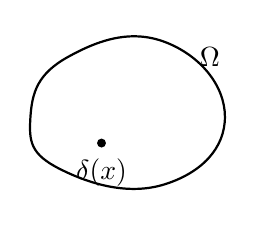
\begin{tikzpicture}[scale=0.95]
  \draw[black, thick]
    plot[smooth cycle, tension=0.8]
    coordinates {(0.15,0.35) (1.55,0.15) (2.35,1.05) (1.55,2.05)
                 (0.25,1.85) (-0.25,1.05)};
  \node[black] at (2.15,1.85) {\(\Omega\)};
  \fill[black] (0.7,0.7) circle (1.7pt);
  \node[below, black] at (0.7,0.62) {\(\delta(x)\)};
\end{tikzpicture}
\end{center}

А что такое \(\delta'(x)\)?
В одномерном случае
\[
\delta'(x)
=
\lim_{h\to 0}
\frac{\delta(x+h)-\delta(x)}{h}.
\]
}

\exr{Разностная производная}{
Показать, что
\[
\widetilde{f}'_{x_i}
=
\lim_{h\to 0}
\frac{\widetilde{f}(x + h e_i) - \widetilde{f}(x)}{h}.
\]
}

\remm{}{
\noindent Вот есть вода --- по сути это \(\rho(x)\):

\begin{center}
\begin{minipage}[t]{0.46\textwidth}
\centering
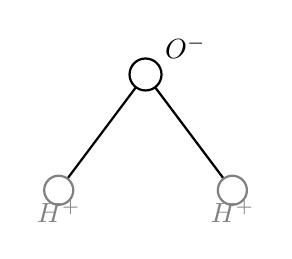
\begin{tikzpicture}[scale=1.05]
  \coordinate (O) at (0,1.55);
  \coordinate (H1) at (-1.05,0.15);
  \coordinate (H2) at (1.05,0.15);
  \draw[thick, black] (O) -- (H1);
  \draw[thick, black] (O) -- (H2);
  \fill[white] (O) circle (5.5pt);
  \draw[thick, black] (O) circle (5.5pt);
  \node[above right, black] at (0.12,1.62) {\(O^-\)};
  \fill[white] (H1) circle (5pt);
  \draw[thick, gray] (H1) circle (5pt);
  \node[below, gray] at (H1) {\(H^+\)};
  \fill[white] (H2) circle (5pt);
  \draw[thick, gray] (H2) circle (5pt);
  \node[below, gray] at (H2) {\(H^+\)};
\end{tikzpicture}
\captionof{figure}{Молекула воды как заряд}
\label{fig:water}
\end{minipage}
\hfill
\begin{minipage}[t]{0.48\textwidth}
\centering
\begin{tikzpicture}[x=1.15cm, y=0.95cm]
  \draw[-{Stealth}, gray!75] (-2.15,0) -- (2.35,0)
        node[right, gray] {\(\R\)};
  \draw[black, thick] (-1.05,0) -- (-1.05,1.45);
  \node[above, black] at (-1.05,1.45) {\(f\)};
  \fill[black] (-1.05,0) circle (2pt);
  \node[below] at (-1.05,-0.08) {\(-h\)};
  \node[above left, black] at (-1.12,0.12) {\(+\delta\)};
  \draw[black, thick] (0,0) -- (0,-1.15);
  \fill[black] (0,0) circle (2pt);
  \node[below left, black] at (-0.05,-1.15) {\(-\delta\)};
  \node[above right] at (0.08,0.05) {\(0\)};
  \draw[gray!60] (-2.0,1.85) .. controls (-0.4,1.55) and (0.7,1.95) .. (2.15,1.75);
\end{tikzpicture}
\captionof{figure}{Диполь: \(+\delta\) и \(-\delta\)}
\label{fig:dipole}
\end{minipage}
\end{center}

Расстояние между атомами точно определить нельзя, поэтому физики
обозначают это \(D\delta\) --- диполь.

Пусть \(S\) --- двусторонний слой, \(\nu \in L_1(S)\). Тогда
\[
\Bigl\langle
    -\frac{\partial}{\partial \vec{n}}\, \nu\, dS,\,
    \phi
\Bigr\rangle
=
\int_S \nu(x)\,
\frac{\partial \phi}{\partial \vec{n}}(x)\,
dS_x.
\]
}

\ex{Сингулярное ядро на прямой}{
Пусть \(n=1\), \(A \in C\),
\(\displaystyle \int_{S_1} A = 0\),
то есть \(A(1)+A(-1)=0\).
Тогда \(A = c \cdot \sgn(x)\) и
\[
\Pvf \frac{A\bigl(\tfrac{x}{|x|}\bigr)}{|x|}
=
c \cdot \Pvf \frac{\sgn(x)}{|x|}.
\]
Это все сингулярные ядра в \(\R\).
}

% =====================================================================
\subsection{Прямое произведение обобщённых функций}

Давайте предположим, что существует коммутативное, ассоциативное произведение обобщённых функций, согласованное с обычным умножением на
\(C^\infty\)- функции.
Тогда рассмотрим произведение
\(\delta(x) \cdot x \cdot \Pvf\frac{1}{x}\)
в двух ассоциациях.

\begin{align*}
\bigl(\delta(x) \cdot x\bigr)\, \Pvf\frac{1}{x}
&=
\bigl(\underbrace{x\,\delta(x)}_{=0}\bigr)\,
\Pvf\frac{1}{x}
= 0.
\end{align*}

С другой стороны, сначала перемножим \(x\) и главное значение:
\begin{align*}
\Bigl\langle x\, \Pvf\frac{1}{x},\, \phi \Bigr\rangle
&=
\Bigl\langle \Pvf\frac{1}{x},\, x\phi \Bigr\rangle
=
\int_{-R}^{R}
    \frac{x\phi(x) - 0\cdot\phi(0)}{x}\,dx
=
\int_{-R}^{R} \phi(x)\,dx
=
\langle 1,\, \phi \rangle.
\end{align*}
\stat{Промежуточный факт}{
\[
x\, \Pvf\frac{1}{x} = 1.
\]
}
Отсюда
\(\delta(x) \cdot \bigl(x\, \Pvf\frac{1}{x}\bigr)
= \delta(x) \cdot 1 = \delta(x)\),
а не ноль. Следовательно, такого умножения быть не может.

\exr{Дизъюнктные носители}{
Если \(\supp f \cap \supp g = \varnothing\), то такое произведение
определить можно.
}

Можно умножать функции \emph{различных} переменных:
\[
f(x) \in L_1^{\loc}(\Omega_1),
\qquad
g(y) \in L_1^{\loc}(\Omega_2),
\]
где \(\Omega_1 \subset \R^n\) и \(\Omega_2 \subset \R^m\).
Тогда \(f(x)g(y) \in L_1^{\loc}(\Omega_1 \times \Omega_2)\) и
\begin{align*}
\bigl\langle
    f(x)g(y),\,
    \underbrace{\phi(x,y)}_{\in C_0^\infty(\Omega_1\times\Omega_2)}
\bigr\rangle
&=
\int_{\Omega_1\times\Omega_2}
    f(x)g(y)\, \phi(x,y)\, dx\, dy \\
&=
\text{(Фубини)}
=
\int_{\Omega_1}
    f(x)
    \Biggl(
        \int_{\Omega_2} g(y)\, \phi(x,y)\, dy
    \Biggr) dx \\
&=
\bigl\langle
    f(x),\,
    \langle g(y),\, \phi(x,y) \rangle
\bigr\rangle.
\end{align*}
Этой же формулой мы хотим определить прямое произведение
в общем случае.

\dfn{Прямое произведение}{
\[
\langle f(x)g(y),\, \phi(x,y) \rangle
=
\langle f(x),\, \langle g(y),\, \phi(x,y) \rangle \rangle.
\]
}

\stat{Корректность}{
Эта формула корректно определяет обобщённую функцию в
\(\DD'(\Omega_1 \times \Omega_2)\).
}

\prf{
Надо проверить, что
\begin{enumerate}[leftmargin=1.6em,itemsep=3pt]
    \item функция
    \(\psi(x) := \langle g(y),\, \phi(x,y) \rangle\)
    лежит в \(\DD(\Omega_1)\) --- проверка корректности;
    \item отображение
    \(\phi \mapsto
    \langle f(x),\, \langle g(y),\, \phi(x,y) \rangle \rangle\)
    непрерывно по \(\phi \in \DD(\Omega_1 \times \Omega_2)\).
\end{enumerate}

\noindent\textbf{Пункт 1.}
Пусть \(\widetilde{\phi}_x(y) := \phi(x,y) \in C_0^\infty(\Omega_2)\).
Тогда
\[
\supp \widetilde{\phi}_x
\subset
\Pi_y(\supp \phi),
\]
и как непрерывный образ компакта множество
\(\Pi_y(\supp \phi)\) компактно, поэтому
\(\widetilde{\phi}_x\) финитна.

\begin{center}
\begin{tikzpicture}[x=1.15cm, y=1.05cm]
  \draw[-{Stealth}, gray!70] (-0.3,0) -- (4.3,0)
        node[right] {\(\Omega_1\)};
  \draw[-{Stealth}, gray!70] (0,-0.25) -- (0,3.15)
        node[above] {\(\Omega_2\)};
  \draw[black, thick]
    plot[smooth cycle, tension=0.7]
    coordinates {(1.15,0.95) (2.85,0.85) (3.25,1.85)
                 (2.35,2.45) (1.25,2.15)};
  \node[black] at (2.2,1.65) {\(\supp\phi\)};
  \draw[gray, densely dashed] (1.15,0) -- (1.15,0.95);
  \draw[gray, densely dashed] (3.25,0) -- (3.25,1.85);
  \draw[{Stealth}-{Stealth}, gray]
        (1.15,-0.22) -- (3.25,-0.22);
  \node[below, gray, font=\small] at (2.2,-0.22)
        {\(\Pi_x(\supp\phi)\)};
  \fill[black] (0,0) circle (1.5pt);
\end{tikzpicture}
\captionof{figure}{Носитель \(\phi\) и его проекция}
\label{fig:supp}
\end{center}

\noindent Далее нужно проверить, что \(\psi\) непрерывна по \(x\):
доказательство на следующей паре\ldots
}

\pagebreak
\section{Практика 3}
\renewcommand{\notesheader}{Математическая физика \(\cdot\) Практика 3 \(\cdot\) 18.09}
% =====================================================================

Продолжаем доказательство утверждения.

\stat{}{
\[
\langle f(x)\cdot g(y),\, \phi(x,y) \rangle
:=
\langle f(x),\, \langle g(y),\, \phi(x,y) \rangle \rangle
\]
--- функционал из \(\DD'(\Omega_1\times\Omega_2)\)
(для \(f\in\DD'(\Omega_1)\), \(g\in\DD'(\Omega_2)\)).
}

\prf{
Запись корректна: доказать, что \(\psi\in\DD(\Omega_1)\).

\noindent\textbf{Пункт 1.}
\(\psi(x) := \langle g(y),\, \phi(x,y) \rangle\),
\(\widetilde\phi_x(y)\in C_0^\infty(\Omega_2)\).

\noindent\textbf{Пункт 2.}
\(\psi(x)\) непрерывна при \(x_k\to x_0\):
\[
\psi(x_k)-\psi(x_0)
=
\langle g(y),\,
\widetilde\phi_{x_k}(y)-\widetilde\phi_{x_0}(y) \rangle.
\]
Достаточно доказать, что
\(\widetilde\phi_{x_k}-\widetilde\phi_{x_0}\to 0\) в \(\DD(\Omega_2)\).
\[
\supp\widetilde\phi_x\subset\Pi_y(\supp\phi),
\]
\[
\supp(\widetilde\phi_{x_k}-\widetilde\phi_{x_0})
\subset
\Pi_y(\supp\phi)
\text{ --- общий компакт.}
\]

\(\dfrac{\partial^\alpha}{\partial y^\alpha}\phi(x,y)\) непрерывно на \(\supp\phi\),
\[
\frac{\partial^\alpha}{\partial y^\alpha}\phi(x_k,y)
\rightrightarrows
\frac{\partial^\alpha}{\partial y^\alpha}\phi(x_0,y).
\]

\noindent\textbf{Пункт 3.}
\(\psi\) дифференцируема и
\[
\psi'_{x_k}
=
\biggl\langle
    g(y),\,
    \frac{\partial}{\partial x_k}\phi(x,y)
\biggr\rangle,
\]
\[
\frac{\psi(x+he_k)-\psi(x)}{h}
=
\biggl\langle
    g(y),\,
    \frac{\widetilde\phi_{x+he_k}(y)-\widetilde\phi_x(y)}{h}
\biggr\rangle.
\]
Достаточно доказать, что
\[
\frac{\widetilde\phi_{x+he_k}-\widetilde\phi_x}{h}
\longrightarrow
\frac{\partial}{\partial x_k}\phi_x(y),
\]
\[
\supp\Biggl(
    \frac{\widetilde\phi_{x+he_k}-\widetilde\phi_x}{h}
\Biggr)
\subset
\Pi_y(\supp\phi),
\]
\[
\frac{
    \dfrac{\partial^\alpha}{\partial y^\alpha}\widetilde\phi_{x+he_k}(y)
    -
    \dfrac{\partial^\alpha}{\partial y^\alpha}\widetilde\phi_x(y)
}{h}
=
\frac{\partial}{\partial x_k}
\frac{\partial^\alpha}{\partial y^\alpha}
\phi_{x+\theta he_k}(y),
\]
где \(\theta\in[0,1]\).

\(\dfrac{\partial}{\partial x_k}
\dfrac{\partial^\alpha}{\partial y^\alpha}\phi(x,y)\)
непрерывны на \(\supp\phi\),
\[
\frac{\partial}{\partial x_k}
\frac{\partial^\alpha}{\partial y^\alpha}
\widetilde\phi_{x+\theta he_k}(y)
\underset{h\to 0}{\rightrightarrows}
\frac{\partial}{\partial x_k}
\frac{\partial^\alpha}{\partial y^\alpha}
\phi_x(y).
\]

По индукции докажем, что \(\psi\in C^\infty\).
Индукционный переход это
\[
\frac{\partial^\beta}{\partial x^\beta}\phi
=
\biggl\langle
    g,\,
    \frac{\partial^\beta}{\partial x^\beta}\phi(x,y)
\biggr\rangle.
\]
Применение пунктов 1 и 2: дифференцируемость
\(\dfrac{\partial^\beta}{\partial x^\beta}\phi\) вместо \(\phi\),
\(\psi(x)\in C_0^\infty(\Omega_1)\).
\[
\langle f(x),\, \langle g(y),\, \phi(x,y) \rangle \rangle.
\]
Достаточно доказать непрерывность
\[
\phi\in\DD(\Omega_1\times\Omega_2)
\longmapsto
\psi\in\DD(\Omega_1).
\]
\[
\psi_k\to 0
\quad\text{в }\DD(\Omega_1\times\Omega_2),
\qquad
\psi_k=\langle g(y),\, \phi_k(x,y) \rangle,
\]
\[
\psi_k\to 0\text{ в }\DD(\Omega_1)?
\]
\[
\supp\psi_k
\subset
\Pi_x(\supp\phi_k)
\subset
\Pi_x(\supp\phi)
\]
--- общий компакт для \(\supp\phi_k\).

Нужно доказать для любого \(\beta\):
\[
\frac{\partial^\beta}{\partial x^\beta}\psi_k
\rightrightarrows 0.
\]
Пусть не так. Тогда \(\forall k\ \exists x_k\):
\[
\Biggl|
\biggl\langle
    g(y),\,
    \frac{\partial^\beta}{\partial x^\beta}\phi_k(x,y)
\biggr\rangle
\Biggr|
>\epsilon,
\]
где
\(\dfrac{\partial^\beta}{\partial x^\beta}\phi_k(x,y)=\phi_k(y)\).
Докажем, что \(\phi_k(y)\to 0\) в \(\DD(\Omega_1)\).
\[
\frac{\partial^\alpha}{\partial y^\alpha}
\widetilde{\widetilde\phi}_k
\rightrightarrows 0,
\qquad
\supp\phi_k\subset\Pi_y(K),
\]
\[
\frac{\partial^\alpha}{\partial y^\alpha}
\frac{\partial^\beta}{\partial x^\beta}
\phi_k(x,y)
\rightrightarrows 0
\ \Longrightarrow\
\frac{\partial^\alpha}{\partial y^\alpha}
\frac{\partial^\beta}{\partial x^\beta}
\phi_k(x_k,y)
\Rightarrow 0.
\]
Мы доказали, что
\[
\langle f(x)g(y),\, \phi(x,y) \rangle
=
\langle f(x),\, \langle g(y),\, \phi(x,y) \rangle \rangle.
\]
}

\stat{Прямое произведение коммутативно}{
\[
\langle f(x),\, \langle g(y),\, \phi(x,y) \rangle \rangle
=
\langle g(y),\, \langle f(x),\, \phi(x,y) \rangle \rangle.
\]
}

\prf{
\(\phi(x,y)=\phi_1(x)\,\phi_2(y)\);
\begin{align*}
\langle f(x),\, \langle g(y),\, \phi_1(x)\phi_2(y) \rangle \rangle
&=
\langle f(x),\, \phi_1(x)\, \langle g(y),\, \phi_2(y) \rangle \rangle \\
&=
\langle g(y),\, \phi_2(y) \rangle\,
\langle f(x),\, \phi_1(x) \rangle
=
\text{правая часть}.
\end{align*}
}

\coroll{}{
Для линейной комбинации \(\phi_k(x)\,\widetilde\phi_k(y)\) тоже верно.
}

Докажем, что линейные комбинации
\(\phi_k(x)\,\widetilde\phi_k(y)\) плотны в \(\DD(\Omega_1\times\Omega_2)\).
\[
\dim\Omega_1=\dim\Omega_2=1.
\]

\exr{}{Доказать для общего случая.}

\[
\phi(x,y)\in\DD(\Omega_1\times\Omega_2),
\qquad
\operatorname{dist}\bigl(\partial(K_1\times K_2),\, \partial\supp\phi\bigr)>\delta_1.
\]
\(\supp\phi\).

\(\phi\) можно приблизить многочленом \(P(x,y)\):
\[
\frac{\partial^k}{\partial x^k}
\frac{\partial^k}{\partial y^k}\phi
- P_k
\le
k - \max\bigl(
    1,\
    \text{меры}(K\times K_2)^{k}
\bigr),
\]
\(x\in(x_0,x_1)\), \(y\in(y_0,y_1)\).

\begin{center}
\begin{tikzpicture}[x=1.05cm, y=1.0cm]
  \draw[-{Stealth}, gray!70] (0,0) -- (5.15,0);
  \draw[-{Stealth}, gray!70] (0,0) -- (0,4.35);
  \node[below, gray] at (4.3,-0.05) {\(\Omega_1\)};
  \node[left, gray] at (-0.05,3.5) {\(\Omega_2\)};
  \draw[black] (0.55,0.45) rectangle (4.55,3.95);
  \draw[black, thick] (1.25,1.05) rectangle (3.45,3.15);
  \node[below left, font=\small] at (1.25,1.05) {\((x_0,y_0)\)};
  \node[above right, font=\small] at (3.45,3.15) {\((x_1,y_1)\)};
  \draw[black, thick]
    plot[smooth cycle, tension=0.75]
    coordinates {(1.7,1.55) (2.55,1.4) (3.1,2.05)
                 (2.75,2.7) (1.95,2.6) (1.55,2.05)};
  \node at (2.35,2.05) {\(\supp\phi\)};
\end{tikzpicture}
\captionof{figure}{Носитель \(\phi\) в прямоугольнике \(\Omega_1\times\Omega_2\)}
\label{fig:supp-rect}
\end{center}

\[
A
=
\Biggl|
\int_{x_0}^{x}\int_{x_0}^{x}\cdots
\int_{y_0}^{y}\int_{y_0}^{y}
\Biggl(
\frac{\partial^k}{\partial x^k}
\frac{\partial^k}{\partial y^k}\phi
- P
\Biggr)
\Biggr|
\le
\frac{\text{меры}(K_1\times K_2)^{k}}
{k\cdot\max\bigl(1,\ \text{меры}(K_1\times K_2)^{k}\bigr)}
\le
\frac{1}{k},
\]
где \(A=|\phi-\widetilde\phi_\kappa|\).

\[
h_1\in C_0^\infty(\Omega_1),
\qquad
h_2\in C_0^\infty(\Omega_2).
\]
\[
h_1\equiv 1\text{ в }\Pi_x\supp\phi,
\]
\[
h_2\equiv 1\text{ в }\Pi_y\supp\phi,
\]
\[
h_1,\, h_2=0\text{ вне }K\times K.
\]
Докажем, что
\(\widetilde P_k(x,y)\, h_1(x)h_2(y)
\xrightarrow[k]{}
\phi\)
в \(\DD(\Omega_1\times\Omega_2)\).
\[
\alpha=(k_1,k_2).
\]
\begin{align*}
D^\alpha(P_k h_1 h_2-\phi)
&=
D^\alpha\bigl(h_1 h_2(\widetilde P_k-\phi)\bigr) \\
&=
\sum_{\beta\le\alpha}
    C_{\beta,\alpha}\,
    D^\beta(h_1,h_2)\,
    D^{\alpha-\beta}(\widetilde P_k-\phi)
\le
\end{align*}
где \(D^\beta(h_1,h_2)\le C_\beta\),
\(D^{\alpha-\beta}(\widetilde P_\kappa-\phi)\le\dfrac{\ell}{k}\),
\[
\le
\Biggl(
    \sum_{\beta\le\alpha} C_{\beta,\alpha} C_\beta
\Biggr)
\cdot\frac{1}{k}
=
\frac{C_\alpha}{k}
\xrightarrow[k]{} 0.
\]
Тут мы просто ввели обозначение:
\(\displaystyle\sum_{\beta\le\alpha} C_{\beta,\alpha} C_\beta = C(\alpha)\).

% ---------------------------------------------------------------------
\subsection{Сходимость обобщённых функций}

\dfn{}{
\[
f_k\to f\text{ в }\DD'(\Omega)
\stackrel{\mathrm{def}}{\Longleftrightarrow}
\forall\phi\in\DD(\Omega)\ \
\langle f_k,\, \phi \rangle
\to
\langle f,\, \phi \rangle.
\]
}

\remm{Литература}{Владимиров, «Уравнения математической физики».}

\thm{}{\(\DD'(\Omega)\) полно.}

\prf{
Если \(\forall\phi\ \langle f_k,\, \phi \rangle\) сходится, то
\[
\langle f,\, \phi \rangle
=
\lim_k\langle f_k,\, \phi \rangle
\]
--- это функционал из \(\DD'(\Omega)\).
}

\noindent\textbf{Упражнения.}

\exr{}{
\(\omega_\epsilon\) --- аппроксимативная единица.
\(\displaystyle\lim_{\epsilon\to 0}\omega_\epsilon\)
(ответ: \(\delta\)-функция).
}

\exr{}{
\(\displaystyle\lim_{h\to 0}\frac{f(x+h)-f(x)}{h}=?\)
(дома).
}

\exr{}{
\(\displaystyle\lim_{\epsilon\to 0}\frac{1}{x+i\epsilon}=?\)
в \(\DD'(\R)\)
(решили на паре).
}

Решим третью.
\[
\biggl\langle
    \frac{1}{x+i\epsilon},\,
    \phi(x)
\biggr\rangle
=
\int_{-A}^{A}\frac{\phi(x)}{x+i\epsilon}\,dx,
\]
где \(\supp\phi\subset[-A,A]\). Домножим на сопряжённое:
\begin{align*}
\int_{-A}^{A}\frac{\phi(x)(x-i\epsilon)}{x^2+\epsilon^2}\,dx
&=
\int_{-A}^{A}\frac{\phi(x)\,x}{x^2+\epsilon^2}\,dx
-
i\epsilon\int_{-A}^{A}\frac{\phi(x)}{x^2+\epsilon^2}\,dx \\
&=
\underbrace{
    \int_{-A}^{A}
        \frac{(\phi(x)-\phi(0))\,x}{x^2+\epsilon^2}\,dx
}_{*}
+
\underbrace{
    \phi(0)\int_{-A}^{A}\frac{x}{x^2+\epsilon^2}\,dx
}_{=\,0\ \text{(нечётная функция)}} \\
&\qquad
-
i\epsilon\int_{-A}^{A}\frac{\phi(x)}{x^2+\epsilon^2}\,dx.
\end{align*}
\[
|*|
\le
\frac{\max|\phi'|\, x^2}{x^2+\epsilon^2}
<
\max|\phi'|,
\]
и получим
\[
\int_{-A}^{A}\frac{\phi(x)-\phi(0)}{x}\,dx
=
\biggl\langle
    \Pvf\frac{1}{x},\,
    \phi
\biggr\rangle
\]
(см.\ практику 2, сингулярные ядра в \(\R\)).
\[
-i\epsilon\int_{-A}^{A}
\frac{
    \phi(0)+\phi'(0)+\dfrac{\phi'(\theta_x)\,x^2}{2}
}{x^2+\epsilon^2}\,dx,
\qquad
\theta_x\in(0,x),
\]
где \(\dfrac{\phi'(0)}{x^2+\epsilon^2}\) нечётно, поэтому остаётся только
\[
-i\epsilon\,\phi(0)\int_{-A}^{A}\frac{dx}{x^2+\epsilon^2}
-
\frac12 i\epsilon
\int_{-A}^{A}
    \frac{\phi'(\theta_x)\,x^2}{x^2+\epsilon^2}\,dx.
\]
\(\dfrac{i\epsilon}{2}\to 0\),
\(\displaystyle\int\frac{\phi'(\theta_x)\,x^2}{x^2+\epsilon^2}
\to\int\phi'(0)\),
в итоге правое слагаемое это просто \(0\).
\[
-i\epsilon\,\phi(0)\int_{-A}^{A}\frac{dx}{x^2+\epsilon^2}
=
-i\epsilon\,\phi(0)\,
\frac{\operatorname{arctg}(x/\epsilon)}{\epsilon}
\Big|_{x=-A}^{x=A}
\longrightarrow
-i\pi\,\phi(0).
\]
Получается
\[
\frac{1}{x+i\epsilon}
\longrightarrow
\Pvf\frac{1}{x}-i\pi\delta.
\]

\exr{}{Доказать это для \(\dfrac{1}{x-i\epsilon}\).}

\remm{}{
\(\phi\in A(\Omega)\),
\[
\int_{\Omega}\frac{\phi(\xi)}{\xi-z}\,d\xi
=
\begin{cases}
2i\pi\,\phi(z), & z\in\Omega_i, \\
0, & z\in\Omega_e.
\end{cases}
\]
\(\phi\in C(C)\),
\(\displaystyle\int_C\frac{\phi(\xi)}{\xi-z}\,d\xi\).
}

\begin{center}
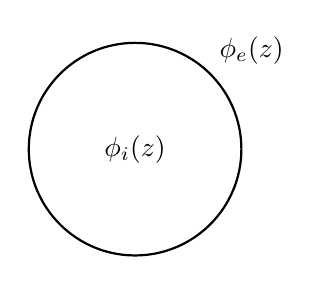
\begin{tikzpicture}[baseline=(current bounding box.center)]
  \draw[black, thick] (0,0) circle (1.35cm);
  \node at (0,0) {\(\phi_i(z)\)};
  \node[above right] at (0.95,0.95) {\(\phi_e(z)\)};
\end{tikzpicture}
\captionof{figure}{Контур: \(\phi_i(z)\) внутри, \(\phi_e(z)\) снаружи}
\label{fig:contour}
\end{center}

\subsection{Формула Сохоцкого}

Общая формула, которую мы по сути доказали: для \(z\in C\)
(то есть для \(z\) из контура)
\begin{align*}
2\pi i\,\phi_e(z)
&=
\vp\int_C\frac{\phi(\xi)}{\xi-z}
+
i\pi\,\phi(z),
\\[4pt]
2\pi i\,\phi_i(z)
&=
\vp\int_C\frac{\phi(\xi)}{\xi-z}
-
i\pi\,\phi(z),
\end{align*}
где \(C=\{\operatorname{Im} z=0\}\). Это формула Сохоцкого.

\begin{center}
\begin{tikzpicture}[x=1.15cm, y=1.05cm]
  \draw[-{Stealth}, gray!70] (0,-1.55) -- (0,1.7)
        node[above] {\(\operatorname{Im} z\)};
  \draw[black, very thick] (-2.35,0) -- (2.55,0);
  \node[right] at (2.55,0) {\(\operatorname{Re} z\)};
  \node at (0.85,0.72) {\(\Omega_e\)};
  \node at (0.85,-0.72) {\(\Omega_i\)};
\end{tikzpicture}
\captionof{figure}{Полуплоскости \(\Omega_e\), \(\Omega_i\) и ось \(\operatorname{Im} z=0\)}
\label{fig:halfplanes}
\end{center}

\[
2\pi i\,\phi_e(0)
=
\phi(0+i\epsilon)
=
\vp\int\frac{\phi(\xi)}{\xi}
-
i\pi\,\phi(0).
\]

\ex{Облучаем частицу}{
\begin{align*}
\int_{-\delta}^{\delta} dE
\int_0^\infty
    f(E)\, e^{-iEt}\, dt
&=
\lim_{\epsilon\to 0}
\int_{-\delta}^{\delta} dE
\int_0^\infty
    f(E)\, e^{-iEt-\epsilon t}\, dt \\
&=
\lim_{\epsilon\to 0}
i\int_{-\delta}^{\delta}
    \frac{f(E)}{E-i\epsilon}\, dE
=
\pi f(0)
-
i\,
\vp\int\frac{f(E)}{E}\, dE.
\end{align*}
}

\exr{}{
\[
\lim_{n\to\infty}
\Pvf\frac{\cos nx}{x}
=?,
\]
\[
\lim_{n\to\infty}
\Pvf\frac{\sin nx}{x}
=?
\]
}

% ---------------------------------------------------------------------
\subsection{Свёртка обобщённых функций}

\[
g,\, f\in L_1(\R^n),
\]
\[
f*g\ (x)
=
\int_{\R^n} f(y-x)\, g(y)\, dy
=
\int_{\R^n} f(y)\, g(y-x)\, dy.
\]

\remm{Напоминание}{
Свёртка порождает на \(L_1\) алгебру, которая называется
свёрточная алгебра.
}

\remm{}{
Если \(*\) --- умножение в \(L_1(\R^n)\), то \(L_1(\R^n)\) ---
это алгебра без единицы.
}

\[
\langle f*g(x),\, \phi(x) \rangle
=
\int_{\R^n}\int_{\R^n}
    f(y-x)\, g(y)\, \phi(x)\, dx\, dy.
\]
Введём \(z=xy\), \((x,y)\to(z,y)\).
\[
\int_{\R^n}\int_{\R^n}
    f(z)\, g(y)\, \phi(z+y)
=
\langle f(z)g(y),\, \phi(z+y) \rangle.
\]

\begin{center}
\begin{tikzpicture}[x=1.05cm, y=1.0cm]
  \draw[-{Stealth}, gray!70] (-0.5,0) -- (4.6,0) node[right] {\(y\)};
  \draw[-{Stealth}, gray!70] (0,-2.05) -- (0,2.25);
  \fill[black] (0,0) circle (1.4pt);
  \node[below left] at (0,0) {\(0\)};
  \draw[black, thick] (0.55,-1.85) -- (2.85,1.95);
  \draw[black, thick] (1.7,-1.85) -- (4.0,1.95);
  \draw[black] (1.35,-0.85) -- (1.95,-0.25);
  \draw[black] (1.85,-0.15) -- (2.45,0.45);
  \draw[black] (2.15,-1.35) -- (2.75,-0.75);
  \draw[black] (2.55,0.35) -- (3.15,0.95);
  \node[below] at (2.15,-0.08) {\(\supp\phi(y)\)};
  \draw[-{Stealth}] (3.55,1.55) -- (2.95,1.15);
  \node[above right] at (3.15,1.45) {\(\supp\phi(z+y)\)};
\end{tikzpicture}
\captionof{figure}{Носители \(\supp\phi(y)\) и \(\supp\phi(z+y)\)}
\label{fig:supp-conv}
\end{center}


\pagebreak
\section{Практика 4}
\renewcommand{\notesheader}{Математическая физика \(\cdot\) Практика 4 \(\cdot\) 25.09}
% =====================================================================

\subsection{Свёртка обобщённых функций (продолжение)}

\(f,g\in L_1(\R^n)\), \(\phi\in\DD(\R^n)\)
\[
\langle f*g,\, \phi \rangle
=
\langle f(x)\, g(y),\, \phi(x+y) \rangle.
\]

\dfn{Последовательность функций, сходящаяся к \(1\)}{
\(\eta_k\in\DD(\Omega)\), \(\eta_k\to 1\), если
\begin{enumerate}[leftmargin=1.6em,itemsep=3pt]
    \item \(\forall\, T\)-компакт в \(\Omega\) \(\exists\, k_0\):
    \(\eta_k\equiv 1\) на \(T\) для всех \(k\ge k_0\);
    \item \(|D^\alpha\eta_k|\le C_\alpha\).
\end{enumerate}
}

\remm{}{\(\eta_k\) --- финитизатор.}

\begin{center}
\begin{tikzpicture}[x=0.85cm, y=0.7cm]
  \draw[-{Stealth}, gray!70] (-3.4,0) -- (3.6,0);
  \draw[-{Stealth}, gray!70] (0,-0.4) -- (0,2.15);
  \draw[black, thick]
    (-3.1,0) .. controls (-2.2,0) and (-1.7,0.15) .. (-1.15,1.15)
    .. controls (-0.75,1.85) and (-0.45,1.85) .. (0.7,1.85)
    .. controls (1.55,1.85) and (1.9,1.7) .. (2.45,0.35)
    .. controls (2.85,0.05) and (3.05,0) .. (3.35,0);
\end{tikzpicture}
\end{center}

\(f,g\in\DD'(\R^n)\), \(\eta_k\) --- финитизатор в \(\R^{2n}\).

\(\langle f(x)g(x),\, \eta_k(x,y)\, \phi(x+y) \rangle\) ---
непрерывный линейный функционал.

Если \(\phi_m\xrightarrow{m} 0\) в \(\DD(\R^n)\), то
\(\eta_k(x,y)\, \phi_m(x+y)\xrightarrow{m} 0\) в \(\DD(\R^{2n})\).

Если \(\exists\lim\limits_k
\langle f(x)g(y),\, \eta_k(x,y)\, \phi(x+y) \rangle\).

\dfn{}{
\[
\langle f*g,\, \phi \rangle
:=
\lim_k
\langle f(x)g(y),\, \eta_k(x,y)\, \phi(x+y) \rangle,
\]
если предел существует и не зависит от финитизатора.
}

Рассмотрим другое возможное определение:
\[
\langle f*g,\, \phi \rangle
=
\iint_{\R^{2n}} f(x)g(y)\, \phi(x+y)\, dx\, dy
= A.
\]
Заметим, что
\[
\iint_{\R^{2n}}
    f(x)g(y)\, \eta_k(x,y)\, \phi(x+y)\, dx\, dy
\xrightarrow{k\to\infty} A
\]
по теореме Лебега (о мажорируемой сходимости).
То есть эти два определения совпадают.

% ---------------------------------------------------------------------
\subsection{Свойства свёртки (если она вообще существует)}

\noindent\textbf{0)}\enspace Коммутативна.

\noindent\textbf{1)}\enspace Линейна по каждому множителю.

\noindent\textbf{2)}\enspace
\(D^\alpha(f*g)=(D^\alpha f)*g=f*(D^\alpha g)\),
то есть эти свёртки существуют и равны.

\prf{
Достаточно доказать для одной свёртки
(далее по коммутативности) и для одной производной
(далее по индукции).

Пусть \(\eta_k\) --- финитизатор.
\begin{align*}
\langle D_i f*g,\, \phi \rangle
&=
\langle D_i f(x)\, g(y),\, \eta_k(x,y)\, \phi(x+y) \rangle \\
&=
\langle D_i\bigl(f(x)g(y)\bigr),\, \eta_k(x,y)\, \phi(x+y) \rangle \\
&=
-\langle f(x)g(y),\, D_{x_i}\eta_k(x,y)\, \phi(x+y) \rangle \\
&\qquad
-\langle f(x)g(y),\, \eta_k(x,y)\, D_i\phi(x+y) \rangle
= I+II.
\end{align*}
\[
II=\langle D_i(f*g),\, \phi \rangle
\]
\[
I
=
-\langle f(x)g(y),\,
    \bigl(\eta_k(x,y)+D_{x_i}\eta_k(x,y)\bigr)\phi(x+y) \rangle
+
\langle f(x)g(y),\, \eta_k(x,y) \rangle.
\]
Заметим, что
\(\bigl(\eta_k(x,y)+D_{x_i}\eta_k(x,y)\bigr)\) --- тоже финитизатор.

\remm{}{
Если \(\eta_k\equiv 1\) в \(B_R\) для всех \(k\ge k_0\), то
\(D_{x_i}\eta_k\equiv 0\) в \(B_R\), соответственно
\(\eta_k+D_{x_i}\eta_k\equiv 1\) в \(B_R\).
}
\[
|D^\alpha\eta_k|\le C_\alpha,
\qquad
|D^\alpha D_{x_i}\eta_k|\le C_{\alpha+e_i},
\qquad
\bigl|D^\alpha(\eta_k+D_{x_i}\eta_k)\bigr|\le\widetilde C_\alpha.
\]
В итоге получаем:
\(I\xrightarrow{k\to\infty} 0\) и
\(II\xrightarrow{k\to\infty}\langle D_i(f*g),\, \phi \rangle\).
}

\exr{}{
Привести пример, когда \(\exists\, D_i f*g\), \(\exists\, f*D_i g\),
но они не равны.
}

\noindent\textbf{3)}\enspace
\(f(x)*g(x+h)=(f*g)(x+h)\) --- оператор свёртки коммутирует
с оператором сдвига. (Упражнение)

\remm{}{
Если линейный непрерывный оператор в \(\DD'\) коммутирует
с оператором сдвига, то это свёртка с какой-то функцией.
}

\noindent\textbf{4)}\enspace
\(\supp f*g\subset\overline{\supp f+\supp g}\).

\prf{
\(A\subset B\Leftrightarrow A^c\supset B^c\), докажем, что
\[
\bigl(\supp_{\R^n} f*g\bigr)^c
\supset
\Bigl(\overline{\supp_{\R^n} f+\supp_{\R^n} g}\Bigr)^c.
\]
По определению \(\supp f*g\) это максимальное открытое множество,
где \(f*g=0\), поэтому нужно доказать, что
\[
f*g=0
\quad\text{на}\quad
\bigl(\overline{\supp f+\supp g}\bigr)^c.
\]

\remm{}{
Если без замыкания, то \(\supp f+\supp g\) не обязательно
замкнутое множество.
}

\exr{}{
\(\bigl(\overline{\supp f+\supp g}\bigr)^c\) не обязательно открыто.
}

Нужно доказать, что если
\(\supp\phi\cap\bigl(\overline{\supp f+\supp g}\bigr)=\varnothing\),
то \(\langle f*g,\, \phi \rangle=0\).
\[
\langle f*g,\, \phi \rangle
=
\lim_{k\to\infty}
\langle f(x)g(y),\, \eta_k(x,y)\, \phi(x+y) \rangle.
\]
Допишем, что \(\forall\eta\in\DD(\R^{2n})\)
\[
\langle f(x)g(y),\, \eta(x,y)\, \phi(x+y) \rangle=0.
\]
\begin{align*}
\supp_{\R^{2n}_{x,y}} f(x)g(y)
&=
\supp_{\R^n_x} f(x)\times\supp_{\R^n_y} g(y) \\
&=
\supp_{\R^{2n}_{x,y}}\, \eta(x,y)\, \phi(x,y) \\
&\subset
\supp_{\R^{2n}_{x,y}}\, \phi(x+y) \\
&=
\bigl\{
    (x,y)\in\R^{2n}_{x,y}
    \mid
    x+y\in\supp_{\R^n}\phi
\bigr\}.
\end{align*}
Пусть
\(\supp f(x)g(y)\cap\supp\, \eta(x,y)\, \phi(x+y)\ne\varnothing\)
(содержит \((x,y)\)),
\(x\in\supp_{\R^n} f\),
\(y\in\supp_{\R^n} g\)
\(\Rightarrow\)
\(x+y\in\supp_{\R^n} f+\supp_{\R^n} g\).
Значит \(x+y\in\supp_{\R^n}\phi\)
\[
\Rightarrow
x+y\in
\supp\phi\cap\bigl(\supp f+\supp g\bigr)
\subset
\supp\phi\cap\bigl(\overline{\supp f+\supp g}\bigr)
=\varnothing
\]
--- противоречие.
}

\exr{}{
Пример \(f\) и \(g\):
\(\supp f*g\subset\overline{\supp f+\supp g}\).
}

\noindent\textbf{5)}\enspace
\(\operatorname{singsupp} f+g
\subset
\operatorname{singsupp} f+\operatorname{singsupp} g\)
(без доказательства).

\ex{Свёртка с \(\delta\)}{
Свёртка с \(\delta\) всегда существует.
\begin{align*}
\langle f*\delta,\, \phi \rangle
&=
\lim\langle f(x)\delta(y),\, \eta_k(x,y)\, \phi(x+y) \rangle \\
&=
\lim\langle f(y),\, \phi(x)\, \eta_k(y) \rangle
=
\langle f(x),\, \phi(x) \rangle.
\end{align*}
\(f*\delta=\delta\).
}

\exr{}{
Пример того, что:
1)~$*$ не ассоциативна;
2)~$*$ не непрерывна.
}

% ---------------------------------------------------------------------
\subsection{Достаточное условие существования}

\thm{}{
\(f,g\in\DD'(\R^n)\); \(\supp g=K\) --- компакт.
Тогда существует \(f*g\).
}

\prf{
\(\{\eta_k\}\) --- финитизатор.
Пусть \(\eta\equiv 1\) в окрестности \(K\), \(\eta\in\DD(\R^n)\).

\begin{center}
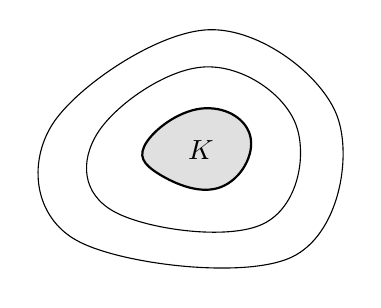
\begin{tikzpicture}[scale=1.05]
  \fill[black!12]
    plot[smooth cycle, tension=0.8]
    coordinates {(-0.55,0.15) (0.15,0.55) (0.7,0.2) (0.35,-0.4) (-0.4,-0.25)};
  \draw[black, thick]
    plot[smooth cycle, tension=0.8]
    coordinates {(-0.55,0.15) (0.15,0.55) (0.7,0.2) (0.35,-0.4) (-0.4,-0.25)};
  \node at (0.1,0.05) {\(K\)};
  \draw[black]
    plot[smooth cycle, tension=0.7]
    coordinates {(-1.15,0.25) (0.15,1.05) (1.25,0.35) (0.85,-0.85) (-0.95,-0.7)};
  \draw[black]
    plot[smooth cycle, tension=0.65]
    coordinates {(-1.7,0.35) (0.2,1.5) (1.75,0.45) (1.2,-1.25) (-1.4,-1.05)};
\end{tikzpicture}
\end{center}

\begin{align*}
\lim\langle f(x)g(y),\, \eta_k(x,y)\, \phi(x+y) \rangle
&=
\lim\langle f(x)\, \eta(y)\, g(y),\, \eta_k(x,y)\, \phi(x+y) \rangle \\
&\qquad\text{(в каком-то упражнении доказали \(\eta g=g\))} \\
&=
\lim\langle f(x)g(y),\, \eta_k(x,y)\, \eta(y)\, \phi(x+y) \rangle \\
&=
\langle f(x)g(y),\, \eta(y)\, \phi(x+y) \rangle.
\end{align*}
Так как \(\eta(y)\phi(x+y)\in\DD(\R^n)\) и, начиная с какого-то \(k\),
\(\eta_k(x,y)\equiv 1\) на \(\supp\eta(y)\, \phi(x+y)\).
\[
\eta(y)\, \phi(x+y)\ne 0,
\qquad
|x+y|\le A,
\]
\[
|y|\le B,
\qquad
|x|\le |x-y+y|\le A+B.
\]

\begin{center}
\begin{tikzpicture}[x=1.05cm, y=0.95cm]
  \draw[-{Stealth}, gray!70] (-0.4,0) -- (4.5,0) node[right] {\(x\)};
  \draw[-{Stealth}, gray!70] (1.3,-1.7) -- (1.3,2.3) node[above] {\(y\)};
  \draw[black, very thick] (1.3,0.15) -- (1.3,1.15);
  \node[below left, font=\small] at (1.15,0.2) {\(\supp\eta(y)\)};
  \node[below left, font=\small, gray] at (0.35,-0.55) {\(\R^n\)};
  \draw[black, thick] (0.2,1.7) -- (3.9,-1.15);
  \draw[black, thick] (1.15,1.7) -- (4.55,-0.85);
  \node[above, font=\small] at (1.55,1.55) {\(\supp\phi(x+y)\)};
  \draw[black] (1.45,1.15) -- (1.85,0.75);
  \draw[black] (1.85,0.7) -- (2.25,0.3);
  \draw[black] (2.2,0.25) -- (2.6,-0.15);
  \draw[black] (2.55,-0.15) -- (2.95,-0.55);
  \node[right, font=\small] at (2.7,0.55) {\(\supp\eta(y)\phi(x+y)\)};
\end{tikzpicture}
\end{center}

\(\supp\, \eta(y)\, \phi(x+y)\) ограничен.
}

\exr{}{
Если \(\supp g\) компакт, то \(f*g\) непрерывна по \(f\).
Если \(g_k\to g\) и \(\supp g_k\subset K\) --- компакт, то \(f*g_k\to f*g\).
}

Пусть \(C\subset\R^n\) --- конус
(то есть множество, для которого \(\forall t>0\) \(tC\subset C\)) такой, что
\begin{enumerate}[leftmargin=1.6em,itemsep=3pt]
    \item \(C\) выпуклый;
    \item \(C\) замкнутый;
    \item \(C\) открытый, \(\operatorname{Int} C^*\ne\varnothing\).
\end{enumerate}
Сопряжённый конус:
\(C^*=\{x\in\R^n\mid (x,y)\ge 0\ \forall y\in C\}\).

\ex{}{
\(C=\R^{n-1}_+=\R^{n-1}\times\R_+\),
тогда \(C^*=\{0\}^{n-1}\times\R_+\).
}

\remm{Для выпуклых конусов}{
\(C\) открытый, \(\operatorname{Int} C^*\ne\varnothing
\Leftrightarrow
C\) не содержит прямых.
}

\thm{}{
Если \(C\) удовлетворяет 1), 2), 3) и
\(f,g\in\DD'(\R^n)\),
\(\supp f\subset C\), \(\supp g\subset C\),
тогда \(\exists\, f*g\) и \(\supp(f*g)\subset C\).
}

\begin{center}
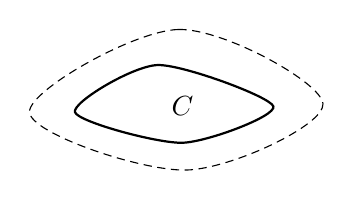
\begin{tikzpicture}[scale=1.05]
  \draw[black, densely dashed]
    plot[smooth cycle, tension=0.55]
    coordinates {(-1.7,0.15) (0.1,1.15) (1.85,0.25) (0.2,-0.55)};
  \draw[black, thick]
    plot[smooth cycle, tension=0.45]
    coordinates {(-1.15,0.15) (-0.15,0.72) (1.25,0.22) (0.15,-0.22)};
  \node at (0.15,0.22) {\(C\)};
\end{tikzpicture}
\end{center}

\[
\eta\equiv 1\text{ в }(C+B_\epsilon(0)),
\quad
\eta\in C^\infty,
\]
\[
\eta=0\text{ вне }(C+B_{2\epsilon}(0)).
\]
\[
\langle f(x)g(y),\, \eta_k(x,y)\, \phi(x+y) \rangle
=
\langle f(x)g(y),\, \eta(x)\eta(y)\, \phi(x+y)\eta_k \rangle.
\]
Если доказать, что
\(\eta(x)\eta(y)\, \phi(x+y)\in\DD(\R^{2n})\),
\[
\lim_k\langle\ldots\rangle
=
\langle f(x)g(y),\, \eta(x)\eta(y)\, \phi(x+y) \rangle\ldots
\]

\ex{}{
\(C\) удовлетворяет 1)--3) и \(C\subset\R\):

\begin{center}
\begin{tikzpicture}[x=0.9cm, y=0.7cm, baseline=(current bounding box.center)]
  \node at (0,0) {\((a)\)};
  \fill (0.85,0) circle (1.6pt);
  \node at (2.3,0) {\((b)\)};
  \fill (3.05,0) circle (1.6pt);
  \draw[black, thick] (3.05,0) -- (4.7,0);
  \node at (6.15,0) {\((c)\)};
  \draw[black, thick] (6.9,0) -- (8.55,0);
  \fill (8.55,0) circle (1.6pt);
\end{tikzpicture}
\end{center}

\((a)\) --- точка, \((b)\) --- луч, \((c)\) --- луч (в обратную сторону).
}

Для \(\R^n\): от противного.
Пусть \(\exists\, (x_k,y_k)\to\infty\),
\[
\eta(x_k)\cdot\eta(y_k)\cdot\phi(x_k+y_k)\ne 0
\Rightarrow
x_k\in C+B_{2\epsilon},\
y_k\in C+B_{2\epsilon},
\]
\[
|x_k+y_k|\le A.
\]
\(x_k\to\infty\), \(y_k\to\infty\), действительно
\[
|x_k+y_k|\le A
\quad\text{и}\quad
|x_k|-|y_k|\le |x_k+y_k|\le A
\quad\text{и}\quad
|y_k|-|x_k|\le |x_k+y_k|<A,
\]
и более того \(\dfrac{|x_k|}{|y_k|}\to 1\).
Ну если это не так, то с какого-то \(k\)
\[
\frac{|x_k|}{|y_k|}\ge 1+\delta
\Rightarrow
|x_k|\ge(1+\delta)|y_k|\ldots,
\]
а у нас \(|x_k|-|y_k|\le |x_k+y_k|\le A\),
а тут \(|x_k|-|y_k|\to\infty\). Противоречие.
\[
\frac{x_k}{|x_k|},\
\frac{y_k}{|y_k|}
\in S_1^{n-1}.
\]
Не умаляя общности
\[
\frac{x_k}{|x_k|}\to\hat x\in S_1,
\qquad
\frac{y_k}{|y_k|}\to\hat y\in S_1.
\]
\[
x_k\in C+B_{2\epsilon},
\quad
\frac{x_k}{|x_k|}
\in
C+B_{2\epsilon/|x_k|}
\Rightarrow
\hat x\in C.
\]
\(\hat y\in C\). (Упражнение)

\[
\hat x+\hat y
\leftarrow
\frac{x_k}{|x_k|}+\frac{y_k}{|y_k|}
=
\underbrace{\frac{x_k+y_k}{|x_k|}}_{\to 0}
+
\underbrace{\frac{y_k}{|y_k|}}_{\text{огр}}
\underbrace{\Bigl(1-\frac{|y_k|}{|x_k|}\Bigr)}_{\to 0}
\to 0,
\]
\(\hat x=-\hat y\), значит \(C\) не открытый --- противоречие.

Осталось доказать, что
\[
\supp f*g
\subset
\overline{\supp f+\supp g}
\subset
\overline{C+C}.
\]
Заметим, что \(C+C=C\), так как если \(x,y\in C\), то
\(\dfrac{x+y}{2}\in C\)
\(\Rightarrow\)
\(2\cdot\dfrac{x+y}{2}=x+y\in C\).

Значит \(\supp f*g\subset C\).

\remm{}{
В конусе \(\DD'(C)\) \(*\) образует алгебру с коммутативным,
ассоциативным умножением и с единицей \(\delta\).
}


\pagebreak
\section{Практика 5}
\renewcommand{\notesheader}{Математическая физика \(\cdot\) Практика 5 \(\cdot\) 02.10}
% =====================================================================

На самом деле утверждение с прошлой пары о том, что
\[
\operatorname{singsupp} f*g
\subset
\operatorname{singsupp} f+\operatorname{singsupp} g
\]
не было верным для нашего определения свёртки.

\dfn{Владимир}{
\(f*g\) существует, если существует
\[
\lim\langle f(x)g(y),\, \eta_k(x,y)\, \phi(x+y) \rangle
\]
и предел не зависит от \(\{\eta_k\}\).
}

Это утверждение будет верным для другого определения свёртки.

\dfn{Хёрмандер}{
\(f*g\) существует, если для всякого компакта \(K\subset\R^n\) множество
\[
S_K
=
\bigl\{
    (x,y)\in\supp f\times\supp g
    \bigm|
    x+y\in K
\bigr\}
\]
ограничено (значит, компактно).
}

\stat{Хёрмандер \(\Rightarrow\) Владимир}{}
\prf{
\(\{\eta_k\}\), \(K=\supp\phi\), \(S_K\) --- компакт,
\(\eta \equiv 1\) на \(K\), \(\eta \in \DD(\R^n)\).
$$\lim\langle f(x)g(y),\, \eta_k(x,y)\, \phi(x+y) \rangle, \quad \phi(x+y)\in C^\infty(\R^{2n}_{x,y}),$$ где $\supp\bigl(\phi(x+y)\, f(x)\, g(y)\bigr)
= S_K\text{ --- компакт}.$ Так что, получаем:
$$
\lim\langle \phi(x+y)\, f(x)\, g(y),\, \eta_k(x,y) \rangle=\lim\langle
    \eta(x,y)\, \phi(x+y)\, f(x)\, g(y),\,
    \eta_k(x,y)
\rangle = $$
$$
=
\lim\langle
    f(x)\, g(y),\,
    \eta_k(x,y)\, \eta\, \phi(x+y)
\rangle = \langle f(x)\, g(y),\, \eta\, \phi(x+y) \rangle.$$
}

\exr{}{Владимир \(\nRightarrow\) Хёрмандер.}

\exr{}{
\(\operatorname{singsupp} f*g
\subset
\overline{\operatorname{singsupp} f+\operatorname{singsupp} g}\)
для Хёрмандера.
}

% ---------------------------------------------------------------------
\subsection{Усреднение обобщённых функций}

\[
\omega(r)=e^{-1/(1-r^2)}
\]
\[
\omega_\epsilon(x)
=
\frac{1}{\epsilon}\,
\omega\Bigl(\frac{|x|}{\epsilon}\Bigr)
\]

\begin{center}
\begin{tikzpicture}[x=1.15cm, y=0.85cm]
  \draw[-{Stealth}, gray!70] (-2.4,0) -- (2.6,0) node[right] {\(r\)};
  \draw[-{Stealth}, gray!70] (0,-0.45) -- (0,2.15);
  \node[below] at (-1,0) {\(-1\)};
  \node[below] at (1,0) {\(1\)};
  \draw[black, thick]
    (-2.2,0) -- (-1,0)
    .. controls (-0.55,0) and (-0.45,1.7) .. (0,1.75)
    .. controls (0.45,1.7) and (0.55,0) .. (1,0)
    -- (2.35,0);
\end{tikzpicture}
\end{center}

Для всех \(f\in\DD'(\R^n)\) свёртка \(f*\omega_\epsilon\) существует.

\remm{}{
\(\operatorname{singsupp}\omega_\epsilon=\varnothing
\Rightarrow
\operatorname{singsupp} f*\omega_\epsilon\subset\varnothing\).
}

\stat{}{\(f*\omega_\epsilon\in C^\infty(\R^n)\).}

\prf{
\(\langle f*\omega,\, \phi \rangle=\)
(в достаточном условии существования свёртки была формула)
\(=\langle f(x)\, \omega_\epsilon(y),\, \eta_\epsilon(x,y)\, \phi(x+y) \rangle\).

\(\eta_\epsilon\equiv 1\) на \(\supp\omega_\epsilon\),
\(\eta_\epsilon\in\DD(\R^n)\).
\begin{align*}
&=
\bigl\langle
    f(x),\,
    \bigl\langle
        \omega_\epsilon(y),\,
        \eta_\epsilon(x,y)\, \phi(x+y)
    \bigr\rangle
\bigr\rangle \\
&=
\Bigl\langle
    f(x),\,
    \int_{\R^n}
        \omega_\epsilon(y)\, \eta_\epsilon(x,y)\, \phi(x+y)\, dy
\Bigr\rangle,
\end{align*}
где \(\omega_\epsilon(y)\, \eta_\epsilon(x,y)=\omega_\epsilon(y)\).

Введём замену под интегралом: \(z=x+y\). Получим
\[
=
\Bigl\langle
    f(x),\,
    \int_{\R^n} \omega_\epsilon(z-x)\, \phi(z)\, dz
\Bigr\rangle.
\]
Далее трюк:
\[
=
\bigl\langle
    f(x)\, \mathds{1}(z),\,
    \omega_\epsilon(z-x)\, \phi(z)
\bigr\rangle,
\]
где \(\mathds{1}(z)\) действует как интеграл, то есть как
\(L_1^{\loc}\)-функция.

Получаем
\begin{align*}
&=
\Bigl\langle
    \mathds{1}(z),\,
    \bigl\langle f(x),\, \omega_\epsilon(z-x)\, \phi(z) \bigr\rangle
\Bigr\rangle \\
&=
\int_{\R^n}
    \bigl\langle f(x),\, \omega_\epsilon(z-x) \bigr\rangle
    \phi(z)\, dz
\end{align*}
и обозначим
\(\langle f(x),\, \omega_\epsilon(z-x) \rangle=h(z)\in C^\infty\):
\[
=
\int_{\R^n} h(z)\, \phi(z)\, dz.
\]
Вспомнили теорему с доказательством корректности прямого произведения,
где показали, что функция вида
\(\langle f(x),\, \omega_\epsilon(z-x) \rangle\in C^\infty\).

Получили, что \(f*\omega_\epsilon=h(z)\in C^\infty\).
}

Введём обозначение \(f_\epsilon=f*\omega_\epsilon\).

\stat{}{\(f_\epsilon\to f\) в \(\DD'(\R^n)\).}

\prf{
\(f*g_k\to f*g\), если \(\supp g_k\subset K\), \(g_k\to g\).

Это было упражнением на одной из прошлых пар, из него всё следует:
\(\omega_\epsilon\to\delta\),
\(f_\epsilon\to f*\delta=f\).
}

\remm{}{
\(\DD'(\R^n)\) --- это на самом деле замыкание
(то есть пополнение) основных функций \(\DD(\R^n)\),
рассматриваемых как функционалы над \(\DD(\R^n)\),
в \(*\)-слабой топологии.
}

\thm{}{
Если \(D^\alpha f=0\) для всех \(|\alpha|=\ell\) в \(\Omega\),
то на самом деле \(f\) --- многочлен степени \(\le\ell-1\) на \(\Omega\).
}

\remm{}{
Для обычных функций это очевидно, теперь же докажем для обобщённых.
}

\prf{
Если доказать, что для всякого \(x\in\Omega\) существует
\(B_\delta(x)\subset\Omega\), в котором \(f=P_{x,\delta}\)
(полином, который может зависеть и от \(x\), и от \(\delta\)).

\begin{center}
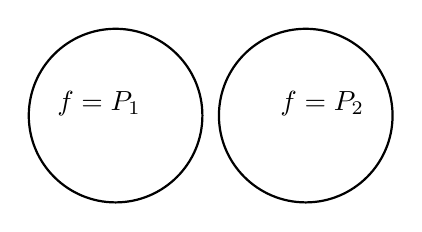
\begin{tikzpicture}[scale=1.05]
  \draw[black, thick] (-1.15,0) circle (1.05cm);
  \draw[black, thick] (1.15,0) circle (1.05cm);
  \node at (-1.35,0.15) {\(f=P_1\)};
  \node at (1.35,0.15) {\(f=P_2\)};
\end{tikzpicture}
\end{center}

Если показали, что в \(B_1\) \(f=P_1\), а в \(B_2\) \(f=P_2\),
то в \(B_1\cap B_2\) \(f=P_1\) и \(f=P_2\). Значит \(P_1\equiv P_2\).

\begin{center}
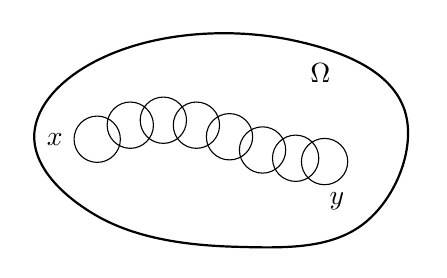
\begin{tikzpicture}[scale=1.05]
  \draw[black, thick]
    plot[smooth cycle, tension=0.7]
    coordinates {(-2.3,0.2) (-1.2,1.15) (0.8,1.25) (2.15,0.45)
                 (1.7,-0.95) (0.1,-1.25) (-1.6,-0.85)};
  \node at (1.15,0.85) {\(\Omega\)};
  \foreach \p in {(-1.55,0.05),(-1.15,0.22),(-0.75,0.28),(-0.35,0.22),
                  (0.05,0.08),(0.45,-0.08),(0.85,-0.18),(1.2,-0.22)}{
    \draw[black] \p circle (0.28cm);
  }
  \node[left] at (-1.85,0.05) {\(x\)};
  \node[below] at (1.35,-0.48) {\(y\)};
\end{tikzpicture}
\end{center}

Возьмём \(x\in\Omega\) и \(B_\delta(x)\subset\Omega\).
Тогда возьмём \(\eta\equiv 1\) в \(B_\delta\) и \(\eta\in\DD(\Omega)\).

Существует \(f\eta\in\DD'(\R^n)\): \(\phi\in\DD(\R^n)\),
\[
\langle f\eta,\, \phi \rangle=\langle f,\, \eta\phi \rangle,
\]
где \(f\in\DD'(\Omega)\), \(\eta\phi\in\DD(\Omega)\),
\(\eta f=f\) в \(B_\delta\).

Существует \((f\eta)_\epsilon\in C^\infty(\R^n)\),
\[
D^\alpha(f\eta)=(D^\alpha f\eta)_\epsilon
\qquad
\forall\, |\alpha|=\ell.
\]
Так как раньше уже говорили, что для свёртки
\(D^\alpha(f*g)=(D^\alpha f)*g=f*(D^\alpha g)\).

\(D^\alpha f\eta=D^\alpha f=0\) в \(B_\delta\).
\begin{align*}
\supp D^\alpha f\eta
&\subset B_\delta^c, \\
\supp D^\alpha(f\eta)_\epsilon
&\subset
\overline{\supp D^\alpha f\eta+B_\epsilon(0)}
\subset
\overline{B_\delta^c+B_\epsilon(0)} \\
&\subset
B_{\delta-\epsilon}(x)
\subset
B_{\delta/2}^c(x).
\end{align*}
Считая, что \(\epsilon<\delta/2\), получаем:
\(D^\alpha(f\eta)_\epsilon=0\) в \(B_{\delta/2}(x)\) ---
это \(C^\infty\)-функция.

Значит \((f\eta)_\epsilon=P_\epsilon\in\mathcal{P}^{\ell-1}\)
в \(B_{\delta/2}\).

Сделаем трюк: на пространстве полиномов \(\mathcal{P}^{\ell-1}\)
введём скалярное произведение
\[
(P_1,P_2)
:=
\int_{\R^n}
    P_1(y)\, P_2(y)\, \omega_{\delta/2}(y-x)\, dy,
\]
где вместо \(\omega_{\delta/2}(y-x)\in\DD(B_\delta)\) могла бы подойти
и любая другая из \(\DD(B_{\delta/2})\).

Тогда мономы \(\{y^\beta\}_{|\beta|\le\ell-1}\) образуют базис
на пространстве полиномов \(\mathcal{P}^{\ell-1}\).
А из алгебры существует дуальный базис для этого скалярного произведения.
То есть существует \(\{\psi_\gamma\}_{|\gamma|\le\ell-1}\) --- базис
\(\mathcal{P}^{\ell-1}\)
(так как \(\mathcal{P}^{\ell-1}\) конечномерно) и
\[
(y^\beta,\psi_\gamma)=\delta_{\beta,\gamma}
\quad\text{(дельта-функция Кронекера)}.
\]
\[
(y^\beta,\psi_\gamma)
=
\int_{\R^n} y^\beta\, \psi_\gamma(y)\, w(y-x)\, dy.
\]
Обозначим \(\psi_\gamma(y)\, w(y-x)=h_\gamma(y)\in C_0^\infty\).

\(\langle(f\eta)_\epsilon,\, h_\gamma\rangle
\to
\langle f\eta,\, h_\gamma\rangle\)
с одной стороны, а с другой
\begin{align*}
\langle(f\eta)_\epsilon,\, h_\gamma\rangle
&=
\langle P_\epsilon,\, h_\gamma\rangle
=
\sum_{|\beta|\le\ell-1}
    C_{\beta,\epsilon}\,
    \langle y^\beta,\, h_\epsilon(y) \rangle
=
C_{\gamma,\epsilon},
\end{align*}
где \(P_\epsilon=\sum_{|\beta|\le\ell-1} C_{\beta,\epsilon}\, y^\beta\).

Таким образом \(C_\gamma:=\langle f\eta,\, h_\gamma\rangle\).
\[
P=\sum_{|\beta|\le\ell-1} C_\beta\, y^\beta.
\]
\(C_{\beta,\epsilon}\to C_\beta
\Rightarrow
P_\epsilon\to P\) в \(L^1_{\mathrm{loc}}(\R^n)\)
и тем более в \(\DD'(B_{\delta/2})\).

Таким образом получили, что в \(\DD(B_{\delta/2})\)
\[
\begin{aligned}
P_\epsilon
&\to P \\
&\parallel \\
(f\eta)_\epsilon
&\to f\eta.
\end{aligned}
\]
То есть \(P=f\eta=f\) в \(B_{\delta/2}\).
Следовательно нашли шар, в котором наша функция есть полином,
что и требовалось.
}

% ---------------------------------------------------------------------
\subsection{Фундаментальное решение дифференциального оператора}

Пусть есть дифференциальный оператор \(L=P(D)\).

Рассматриваем уравнение \(Lu=f\) (например \(-\Delta u=f\))
и хотим его решить.

Сначала найдём решение \(Lu=\delta\).
Пусть это решение существует, обозначим его \(\mathcal{E}\).

Рассмотрим \(u_f:=\mathcal{E}*f\) (если существует свёртка):
\[
Lu_f
=
P(D)(\mathcal{E}*f)
=
(P(D)\mathcal{E})*f
=
\delta*f
=f.
\]
То есть, решив одно уравнение \(Lu=\delta\),
сразу имеем тривиальным образом все решения для \(Lu=f\).

\thm{}{
Для всякого полинома \(P\) с постоянными коэффициентами,
для \(L=P(D)\) существует фундаментальное решение.
}

\ex{}{
Хотим решить \(\sum_{k=0}^{n} C_k u^{(k)}=f\).

Надо найти фундаментальное решение
\(\sum_{k=0}^{n} C_k u_{\text{фунд.}}^{(k)}=\delta\).

Общее решение \(=u_{\text{фунд.}}*f\).
}

\exr{}{
\[
\begin{cases}
\sum C_k u^{(k)}=0, \\
u^{(k)}=0\quad\forall k<n-1, \\
u^{(n-1)}=1.
\end{cases}
\]
}

% ---------------------------------------------------------------------
\subsection{Задача Коши для волнового уравнения в терминах обобщённых функций}

\[
\begin{cases}
u_{tt}-a^2\Delta u=f(x,t), & t>0, \\
u\big|_{t=0}=\phi, \\
u_t\big|_{t=0}=\psi
\end{cases}
\qquad
u\in C^2\bigl(\R^n\times\R_{\ge 0}\bigr).
\]
Попробуем вывести уравнение в обобщённых функциях:
\[
U(x,t)
=
\begin{cases}
u(x,t), & t\ge 0, \\
0, & t<0
\end{cases}
\in L^1_{\loc}(\R^n).
\]
\(U\in L^1_{\loc}(\R^n)\Rightarrow U\) --- обобщённая функция.
\begin{align*}
\langle U_{tt}-a^2\Delta U,\, h \rangle
&=
\langle U,\, h_{tt}-a^2\Delta h \rangle \\
&=
\int_{\R^n}\int_0^\infty
    U\, (h_{tt}-a^2\Delta h)\, dt\, dx.
\end{align*}
Воспользуемся формулой интегрирования по частям.

\begin{center}
\begin{minipage}[t]{0.46\textwidth}
\centering
\begin{tikzpicture}[x=0.85cm, y=0.75cm]
  \draw[-{Stealth}, gray!70] (0,-1.7) -- (0,1.9) node[above] {\(x\)};
  \draw[-{Stealth}, gray!70] (-0.4,0) -- (4.2,0) node[right] {\(t\)};
  \draw[black, thick]
    plot[smooth cycle, tension=0.65]
    coordinates {(0.7,0.9) (1.8,1.25) (3.1,0.7) (3.3,-0.35)
                 (2.1,-0.95) (0.85,-0.45)};
  \node at (2.0,0.25) {\(\supp h\)};
\end{tikzpicture}
\end{minipage}
\hfill
\begin{minipage}[t]{0.46\textwidth}
\centering
\begin{tikzpicture}[x=0.85cm, y=0.75cm]
  \draw[-{Stealth}, gray!70] (0,-1.7) -- (0,1.5) node[above] {\(x\)};
  \draw[-{Stealth}, gray!70] (-0.3,0) -- (4.2,0) node[right] {\(t\)};
  \draw[black, thick] (1.15,-0.85) ellipse (1.15cm and 0.42cm);
  \node at (1.15,-0.85) {\(\supp h\)};
\end{tikzpicture}
\end{minipage}
\end{center}

\begin{align*}
&\int_0^\infty\int_{\R^n}
    (u_{tt}-a^2\Delta u)\, h\, dx\, dt
-
\int_{\R^n} u\, h_t\Big|_{t=0}
+
\int_{\R^n} u_t\, h\Big|_{t=0} \\
&=
\int_0^\infty\int_{\R^n}
    f(x,t)\, h(x,t)\, dx\, dt
-
\int_{\R^n}\phi(x)\, h(x,0)\, dx
+
\int_{\R^n}\psi(x)\, h(x,0)\, dx \\
&=
\langle F,\, h \rangle
+
\langle \phi(x)\, \delta'(t),\, h \rangle
+
\langle \psi(x)\, \delta(t),\, h \rangle,
\end{align*}
где
\[
F(x,t)
=
\begin{cases}
f(x,t), & t\ge 0, \\
0, & t<0.
\end{cases}
\]
В итоге получили обобщённую постановку задачи Коши
для волнового уравнения:
\[
U_{tt}-a^2\Delta U
=
F(x,t)+\phi(x)\, \delta'(t)+\psi(x)\, \delta(t)
\]
--- волновое уравнение в обобщённых функциях.

Фундаментальное решение --- это решение
\(U_{tt}-a^2\Delta U=\delta(x,t)\),
то есть \(F=0\), \(\phi=0\), \(\psi\to\delta\):
\[
\begin{cases}
u_{tt}-a^2\Delta u=0, \\
u\big|_{t=0}=0, \\
u_t\big|_{t=0}=\psi.
\end{cases}
\]
То есть если знаем решение, то знаем решение для всех \(\delta\) и всех \(\phi\).

Если \(u\) --- решение исходного, то \(U\) --- решение
\[
U_{tt}-a^2\Delta U
=
F(x,t)+\phi(x)\, \delta'(t)+\psi(x)\, \delta(t).
\]

\exr{}{
Если \(U\) --- решение верхнего уравнения и
\(U\in C^2\bigl(\R^n\times\R_{\ge 0}\bigr)\),
тогда \(u=U\big|_{\{t\ge 0\}}\) --- решение исходного.
}

Для \(n=1\) воспользуемся формулой Даламбера:
\[
u(x,t)=\int_{x-at}^{x+at}\psi(y)\, dy
\]
--- решение для задачи Коши для волнового уравнения:
\[
\begin{cases}
u_{tt}-a^2\Delta u=0, \\
u\big|_{t=0}=0, \\
u_t\big|_{t=0}=\psi.
\end{cases}
\]

Для того, чтобы получить фундаментальное решение, устремим \(\psi\to\delta\), тогда
\[
u(x,t)
\to
\int_{x-at}^{x+at}\delta(y)\, dy
=
\begin{cases}
1, & 0\in(x-at,\, x+at), \\
0, & 0\notin(x-at,\, x+at).
\end{cases}
\]
Что, как нетрудно заметить, есть характеристическая функция.

Таким образом, сейчас мы нестрого показали, что
\[
u=\chi_{[-at,\, at]}(x)
\]
--- фундаментальное решение для волнового уравнения в \(\R^1\).

\end{document}
